% !TeX root = main.tex
\documentclass[12pt, twoside, a4paper, draft]{report}
\usepackage[utf8]{inputenc}
\usepackage[T1]{fontenc}
\usepackage{lmodern}
\usepackage[english]{babel}
\usepackage{amsmath, amssymb, amsfonts}
\usepackage{graphicx, caption, subcaption, float}
\usepackage{booktabs, multirow, tabularx, paralist, makecell, array}
\usepackage[top=2.5cm, bottom=2.5cm, inner=3cm, outer=2.5cm]{geometry}
\usepackage[dvipsnames, table]{xcolor}
\usepackage{ circuitikz }
\usepackage{fancyhdr}
\fancyhf{}
\fancyhead[L]{\nouppercase{\leftmark}}
\fancyhead[R]{\thepage}
\usepackage[colorlinks=true, citecolor=Plum, linkcolor=MidnightBlue]{hyperref}
\usepackage{setspace}
\onehalfspacing
\usepackage{textcomp}
\usepackage{enumitem}
\usepackage{siunitx}
\usepackage[Sonny]{fncychap}
\usepackage{appendix}
\usepackage{media9}
\usepackage{booktabs}
\definecolor{mypurple}{RGB}{129, 61, 156}




\begin{document}

\begin{titlepage}
    \centering

    {\Huge\textbf{Master's Thesis}\par}
    \vspace{1.5cm}

    %\includegraphics[width=0.3cm]{}\par  University logo
    \vspace{1cm}

    {\Large\textbf{Characterization of filtered Cathodic Arc Plasma Processes}}\par
    \vspace{0.5cm}

    {\Large\textbf{Focusing on Mass Spectroscopy and Ion Flux measurements}}\par
    \vspace{0.5cm}

    {\Large Investigation of correlation between ion flux and deposition rate for TiAl and TiAlN thin films}\par
    \vspace{2cm}

    \textbf{Author}\par
    Paul Junk \par
    \vspace{1cm}

    \textbf{Supervisors}\par
    Dr. Yeliz Unutulmazsoy\par
    Dr. Dmitry Kalanov\par
    \vspace{1cm}
    
    \textbf{Institution}\par
    Leibniz Institute of Surface Engineering (IOM)\par
    Leipzig University \par
    \vspace{1.5cm}

    {\large\textbf{Submission Date}}\par
    \today\par
\end{titlepage}
\tableofcontents
\newpage
\section*{\centering{Abstract}}


Titanium aluminum nitride (Ti--Al--N) coatings are widely used in cutting tools and wear-resistant applications, but their industrial deposition typically requires use of external substrate, usually around 400~°C. Cathodic arc deposition offers room-temperature crystallization through energetic bombardment with multiply charged species. However, multiple process parameters are inherently coupled: external magnetic fields simultaneously increase both ion charge states (potential energy) and ion flux, while reactive gases alter plasma composition through charge-exchange collisions. This thesis investigates the TiAlN plasma to decouple the roles of ion flux, ion potential energy, and ion kinetic energy for room-temperature deposition  of TiAlN as a function of magnetic field strength (0--0.25~T), nitrogen pressure (0--0.3~Pa), and spatial position (10--20~cm from the plasma source).\\

Three main diagnostics tools were used to separate energy effects in the plasma process: a Langmuir probe for ion current density, a quartz crystal microbalance for deposited mass, and an energy-resolving mass spectrometer for charge-state-resolved ion energy distributions. Measurements in metallic mode (vacuum) and reactive mode (nitrogen background) characterized the transition from metallic to reactive deposition and quantified the contribution of ionized versus neutral nitrogen species to film growth.\\

The results show that increasing the magnetic field strength can amplify ion flux by up to a factor of eight for the same distance between the source and the measurement spot. In the reactive process, the presence of nitrogen further boosts ion flux, as charge-exchange collisions reduce the number of highly ionized species and increase the proportion of singly ionized species. Ion energy distribution functions measured by energy-resolved mass spectrometry, shift toward lower ionization levels, when operating in reactive mode.\\

This work extends the ion energy decoupling framework established for (V,Al)N coatings to the industrially relevant TiAlN system and demonstrates that ion flux control via magnetic field strength provides a viable route to tailoring film crystallinity without the need of external substrate temperature.


\chapter{Introduction and Literature Review}\label{chap:intro}

\section{Motivation}

Titanium aluminum nitride (Ti$_{1-x}$Al$_x$N) coatings are widely used, as protective coatings, particularly for cutting tools, because of their high hardness (25--35~GPa), thermal stability, and oxidation resistance \cite{paldey2003}. These properties depend on maintaining the metastable cubic B1 crystal structure, which provides superior mechanical performance compared to the thermodynamically wurtzite phase \cite{mayrhofer2006}. Conventional deposition methods, such as magnetron sputtering require substantial substrate heating to achieve dense, crystalline coatings. Cathodic arc deposition offers a key advantage: highly ionized metal plasmas with intrinsic high ion energies enable room-temperature crystallization through energetic condensation \cite{cathodic_arcs}.\\

The challenge is that cathodic arc processes depend on the interplay of several interdependent parameters. Ion energy has two components: kinetic energy from plasma expansion and potential energy from ionization. External magnetic fields can enhance ion charge states and ion flux, the latter increasing by up to an order of magnitude \cite{RN5}. Adding reactive gases such as nitrogen introduces charge-exchange collisions that alter plasma composition \cite{cathodic_arcs}. Understanding how these parameters individually influence film properties remains a fundamental challenge for predictive thin film deposition.

\section{State of the art}

Recent studies have made progress in understanding and decoupling ion energy effects in cathodic arc deposition. Unutulmazsoy et al.\ showed that applying an external magnetic field at the plasma source increases ion charge states (and thus potential energy), while applying a substrate bias adjusts kinetic energy \cite{unutulmazsoy}. Their work on (V,Al)N films demonstrated that crystalline films can be deposited at room temperature through energetic ion bombardment. Unutulmazsoy et al. stated that ``application of an external magnetic field also leads to an enhancement of the ion flux and hence the desired complete decoupling of the potential and kinetic energy effects requires further steps'' \cite{unutulmazsoy}. In their study, the magnetic field not only modified ion charge states but also increased ion flux by up to a factor of 10, making it impossible to isolate the effect of potential energy from that of ion flux intensity.\\


Kalanov et al.\ refined this approach using detailed energy-resolved mass spectrometry and systematic distance variation \cite{decoupling_kalanov_2025}. Their work on (V,Al)N films showed that the enhancement of room-temperature crystallinity correlates primarily with the increase in potential energy input. Notably, applying a DC bias to increase kinetic energy by approximately 30~eV did not produce the same crystallization effect, even though it increased the total ion energy. This demonstrated that potential energy plays a distinct role in promoting film crystallinity. Crucially, Kalanov et al. addressed the flux-energy coupling by varying the source-to-substrate distance from 8 to 20~cm: moving the substrate further away reduced the ion flux while maintaining similar ion charge states and energies, enabling direct comparison of potential energy effects at almost identical flux levels.\\

Despite these advances, key questions remain for extending this framework to other material systems. Both studies explored the effects of activated nitrogen in reactive deposition, which consists of both ionized and neutral (but excited) nitrogen species \cite{cathodic_arcs,bendikt2012}. While Unutulmazsoy et al. \cite{unutulmazsoy} focused on reactive deposition with nitrogen and Kalanov et al. \cite{decoupling_kalanov_2025} examined both metallic and reactive modes, a key question remains unanswered: what fraction of the activated nitrogen (nitrogen participating in the plasma process) consists of neutral species versus ionized species? This distinction is crucial for understanding the relative contributions of ions and neutrals to film growth, particularly in reactive mode where both species can participate in nitride formation.\\

For TiAlN specifically, which benefits from greater natural abundance and lower cost than vanadium-based nitrides, while comparative studies between cathodic arc and magnetron sputtering have shown that ion energy flux significantly affects texture and mechanical properties \cite{karimi_aghda_2023}, the flux-energy decoupling framework established for (V,Al)N has not been applied to this industrially important system.

\section{Objectives}

This thesis addresses above mentioned gaps in literature by systematically investigating the role of ion flux in Ti--Al--N thin film growth via pulsed filtered cathodic arc deposition. The specific objectives are:

\begin{enumerate}
	\item Characterize the ion flux and the total flux (flux of all particles arriving at the substrate) as a functions of external magnetic field strength and distance from the macroparticle filter. Furthermore, analyse the ion energy distributions of individual ionic species.
	
	\item Investigate the sweet spot from metallic to reactive mode by varying nitrogen pressure and quantify how this affects the ion-to-neutral ratio arriving to the substrate.
	
	\item Establish quantitative correlations between ion flux and total flux across the experimental parameter space of magnetic field, nitrogen pressure, and distance from the macroparticle filter.
	
	\item Characterize the crystallinity, film thickness, film composition of deposited TiAlN films at selected process parameters with film properties.
\end{enumerate}

The experimental approach combines multiple in situ plasma diagnostics with ex situ film characterization to extend the framework \cite{unutulmazsoy, decoupling_kalanov_2025} to both reactive mode operation and the industrially relevant TiAlN system. This multi-diagnostic strategy, applied across a systematic parameter space, enables investigation of two key aspects: (1) explore room temperature deposition of TiAlN films, and (2) the combined measurement of ion flux versus total deposited flux to distinguish the contribution of non-ionized activated nitrogen species and forming thin film structure.

\chapter{Theoretical Background}\label{chap:theory}

\section{Plasma Generation and Composition}

\subsection{Cathode Spot Plasma Generation}

Cathodic arc plasmas form at microscopic emission centers, known as cathode spots, on an otherwise cold metal electrode under vacuum. Spot ignition occurs when the local cathode surface, through breakdown of adsorbates or field-enhanced thermionic emission, undergoes a rapid, explosive release of electrons and vaporized metal. During a single spot pulse, a few nanograms of the cathode material rapidly heat up, vaporize, and ionize, producing a dense, quasineutral plasma plume composed mostly of metal ions and electrons. The peak spot current densities reach \(10^{10}\)--\(10^{12}\)\,A\,m\(^{-2}\), far above steady-state thermionic or field emission limits. These microexplosions, termed ectons (explosive electron emission centers), were first described by Mesyats \cite{mesyats1995} and produce localized nanosecond-scale plasma bursts. The arc is sustained by repetitive ecton events occurring at or near the same location \cite[Chap.~3.3--3.4]{cathodic_arcs}.




Key Characteristics of Spot-Generated Plasma:
\begin{compactitem}
    \item High degree of ionization: >90 \% of the ejected metal atoms emerge as ions, a consequence of the extreme power density in the cathode spot \cite[Chap.~3.5]{cathodic_arcs}.
    \item Multiply charged ions: the charge state distributions extend to \(Q=3\)–4 for refractory metals, such as Ti and Al, due to the high electron temperature and density in the spot plasma \cite[Chap.~3.5]{cathodic_arcs}.
\end{compactitem}

Spot ignition and quenching occur on timescales of 10--100\,ns, with each pulse ejecting a fully ionized burst of metal vapour. The sustained arc discharge thus consists of continuously overlapping microplasma pulses, producing a metal-rich, high-flux ion stream well-suited for energetic thin-film deposition.


\begin{figure}[h]
	\centering
	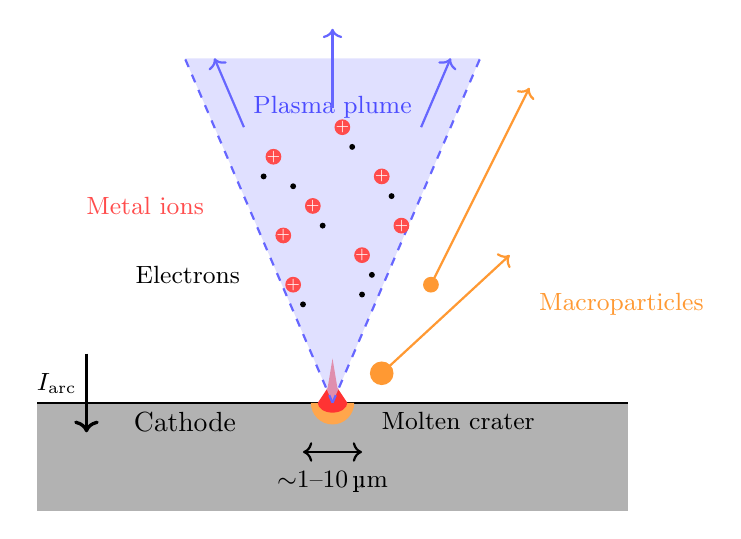
\begin{tikzpicture}[scale=1.25]
		% Cathode block
		\fill[gray!60] (-3,-1.1) rectangle (3,0);
		\draw[thick] (-3,0) -- (3,0);
		\node[below] at (-1.5,0) {Cathode};
		
		% Molten crater
		\fill[orange!70] (-0.22,0) arc (180:360:0.22) -- cycle;
		\fill[red!80] (-0.15,0) arc (180:360:0.15 and 0.1) -- (0.15,0) -- (0.05,0.15) -- (0,0.45) -- (-0.05,0.15) -- (-0.15,0) -- cycle;
		\node[below right, font=\small] at (0.4,0) {Molten crater};
		
		% Plasma plume (expanding cone)
		\fill[blue!20, opacity=0.6] (0,0) -- (-1.5,3.5) -- (1.5,3.5) -- cycle;
		\draw[blue!60, thick, dashed] (0,0) -- (-1.5,3.5);
		\draw[blue!60, thick, dashed] (0,0) -- (1.5,3.5);
		\node[blue!70, font=\small] at (0,3) {Plasma plume};
		
		% Ions (circles with + signs)
		\foreach \x/\y in {-0.4/1.2, 0.3/1.5, -0.2/2.0, 0.5/2.3, -0.6/2.5, 0.1/2.8, 0.7/1.8, -0.5/1.7} {
			\fill[red!70] (\x,\y) circle (0.08);
			\node[white, font=\tiny] at (\x,\y) {+};
		}
		\node[red!70, right, font=\small] at (-2.6,2.0) {Metal ions};
		
		% Electrons (small dots)
		\foreach \x/\y in {-0.3/1.0, 0.4/1.3, -0.1/1.8, 0.6/2.1, -0.7/2.3, 0.2/2.6, -0.4/2.2, 0.3/1.1} {
			\fill[black] (\x,\y) circle (0.03);
		}
		\node[right, font=\small] at (-2.1,1.3) {Electrons};
		
		% Macroparticle (larger droplet trajectory)
		\fill[orange!80] (0.5,0.3) circle (0.12);
		\draw[->, thick, orange!80] (0.5,0.3) -- (1.8,1.5);
		\fill[orange!80] (1,1.2) circle (0.08);
		\draw[->, thick, orange!80] (1,1.2) -- (2,3.2);
		\node[orange!80, right, font=\small] at (2.0,1.0) {Macroparticles};
		
		% Current flow arrow
		\draw[->, very thick] (-2.5,0.5) -- (-2.5,-0.3);
		\node[left, font=\small] at (-2.5,0.2) {$I_{\rm arc}$};
		
		% Spot diameter indicator
		\draw[<->, thick] (-0.3,-0.5) -- (0.3,-0.5);
		\node[below, font=\small] at (0,-0.6) {$\sim$1--10\,\textmu m};
		
		% Expansion arrows
		\draw[->, thick, blue!60] (0,3.0) -- (0,3.8);
		\draw[->, thick, blue!60] (-0.9,2.8) -- (-1.2,3.5);
		\draw[->, thick, blue!60] (0.9,2.8) -- (1.2,3.5);
		
	\end{tikzpicture}
	\caption[Schematic of cathode spot operation]{Schematic of cathode spot operation. The arc current $I_{\rm arc}$ concentrates at a microscopic spot (1--10\,\textmu m diameter), creating a molten crater from which a plasma plume of metal ions, electrons and macroparticles expand. Adapted from \cite{juttner2001}}.
	\label{fig:cathode_spot}
\end{figure}

\subsection{Pulsed vs. Continuous Arc Operation}

Cathodic arcs can operate in either continuous (DC) or pulsed mode, with fundamental differences in plasma generation dynamics. In DC operation, the cathode spot moves continuously across the surface, maintaining a steady-state plasma density determined by the balance between plasma generation at the spot and losses through expansion. The time-averaged plasma properties remain constant, and the ion flux to the substrate is continuous.\\

In pulsed operation, the arc is periodically initiated and extinguished, creating discrete plasma bursts separated by periods with no plasma generation. During the active phase of each pulse, the instantaneous plasma density can be significantly higher than in DC arcs operating at the same average power, because the energy is concentrated in short time intervals. The peak plasma density scales with the instantaneous arc current, which can reach several hundred amperes during the pulse. Between pulses, the plasma expands and dissipates, allowing the cathode surface to cool. This temporal modulation affects both the spot dynamics and the resulting plasma composition.\\

The ion charge state distributions in pulsed arcs are typically similar to or slightly enhanced compared to DC arcs, as the higher instantaneous power density can promote additional ionization events in the cathode spot region \cite[Chap.~10]{cathodic_arcs}. Understanding these temporal plasma dynamics is essential when interpreting flux measurements and correlating them with film growth processes.

\subsection{Plasma Expansion and Macroparticle Filtering}

Following their generation at the cathode spots, the plasma bursts expand into the vacuum chamber. This expansion is supersonic, with ions carrying directed kinetic energy away from the cathode. In many industrial and research systems, the expanding plasma is guided through a magnetic macroparticle filter that removes macroparticles while allowing plasma to pass along curved magnetic field lines.

In the region near the cathode (within a few centimetres of the spot), plasma densities are on the order of \(10^{18}\)\,cm\(^{-3}\) and electron temperatures \(T_e \approx 5\)--10\,eV. As the plume propagates, its density decreases according to
\begin{equation}
	n(r) = \frac{C\,I_{\rm arc}}{r^2}
\end{equation}
where \(I_{\rm arc}\) is the arc current, $r$ the distance, and $C$ a constant related to the ion erosion rate of the cathode material. This \(1/r^2\) scaling assumes free expansion, but deviations can occur due to magnetic fields, collisions, or reactive gases, which may alter the plasma trajectory or cause recombination \cite[Chap.~4.3; Eq.~4.3, p.~178]{cathodic_arcs}.

In cathodic arc discharges from titanium cathodes, whether pure Ti or Ti--Al compounds, ions generally carry an average charge state \(\langle Q\rangle \approx 2.1\)--2.2 at the source \cite[Chap.~4.1; App.~B.8]{cathodic_arcs}. This high degree of ionization reflects the extreme power density of the spot and follows the cohesive energy rule, which links \(\langle Q\rangle\) to the cohesive energy of the cathode material \cite[App.~B.8]{cathodic_arcs}.

In the present work, a 90$^\circ$ curved magnetic filter guides the expanding plasma toward the substrate region while removing macroparticles. After passing through the filter, the plasma has evolved from its initial state at the cathode spot, having undergone expansion, potential collisions with background gas, and interaction with guiding magnetic fields. The properties of this filtered plasma in the substrate region determine the energy and flux delivered to the growing film, and are the focus of the following sections.


%Applying an external axial magnetic field at the source (the “EM-coil” configuration) can boost ⟨Q⟩ by 10–30 \% and increase total ion flux by up to an order of magnitude. Effects attributed to enhanced magnetic insulation and longer plasma spot interaction times \cite{decoupling_kalanov_2025}. In contrast, imposing a DC bias on the source raises the ions’ kinetic energy with minimal change to ⟨Q⟩ or flux, offering a route to decouple kinetic and potential-energy contributions in film-growth studies.\\

\section{Ion Energies and Flux in the Substrate Region}

This section focuses on the properties of ions in the plasma after expansion and filtering, in the region where they reach the substrate and form the growing film.


\subsection{Ion Energies: Origins and Implications}\label{section:ion_energies}

Ions in cathodic arc plasmas carry both kinetic and potential energy. The kinetic energy \(E_{\rm kin}\) arises from the supersonic expansion of plasma from the cathode spot, while the potential energy \(E_{\rm pot}\) is released upon neutralization at the substrate surface and is determined by the ionization states of the ion.

The total energy delivered by an ion to the growing film is
\begin{equation}
	E_{\rm tot} = E_{\rm kin} + E_{\rm pot}.
\end{equation}

For cathodic arc plasmas, the kinetic energy is closely linked to the arc burning voltage, which remains nearly constant at 20--25\,V for most metallic cathodes \cite[Chap.~4.2]{cathodic_arcs}. This voltage accelerates ions away from the cathode region, giving them characteristic drift velocities. As ions traverse the expanding plasma, they may undergo collisions that modify their energy distribution.

Table~\ref{tab:ion_properties} summarizes characteristic ion properties for Ti and Al cathodic arc plasmas in vacuum, measured near the cathode.

\begin{table}[htbp]
	\centering
	\caption[Characteristic ion properties for Ti and Al]{Characteristic ion properties for Ti and Al cathodic arc plasmas in vacuum, near the cathode \cite[App.~B; Table~B.8]{cathodic_arcs}.}
	\label{tab:ion_properties}
	\begin{tabular}{lcccc}
		\toprule
		Species & $\langle Q \rangle$ & $E_{\rm kin}$ (eV) & $E_{\rm pot}$ (eV) & $E_{\rm tot}$ (eV) \\
		\midrule
		Ti$^{2+}$ & 2.1 & 59 & 21 & 80 \\
		Al$^{2+}$ & 1.7 & 28 & 24 & 52 \\
		\bottomrule
	\end{tabular}
\end{table}


These values, measured near the cathode spot, serve as reference for understanding the energy budget of ions. In this work, the plasma is characterized after expansion and filtering, where ion energies may differ from these initial values due to collisions and field effects. Nonetheless, for the materials used in this work, the total ion energies are expected to exceed the approximately 30\,eV threshold for subplantation, enabling densification and improved crystallinity in Ti--Al--N films without requiring external substrate heating \cite[Chap.~8.1--8.2]{cathodic_arcs}.


\subsection{Effect of Distance on Ion Properties}

As ions travel from the cathode through the filter and toward the substrate, their properties evolve due to geometric expansion and potential collisions. The ion flux decreases with the square of the distance due to the expanding plasma front. Additionally, collisions with background gas (if present) can reduce ion kinetic energies and alter charge state distributions through charge-exchange reactions.\\

In vacuum (metallic mode), the ion energy distributions remain relatively narrow and well-defined. At increased distances, the plasma density decreases but the relative composition and charge states are largely preserved. However, the ion flux at the substrate position becomes a critical parameter, as it determines the rate at which energy is delivered to the growing film. Understanding how distance affects the ion flux therefore provides insight into the spatial uniformity of the deposition process and allows optimization of substrate positioning.

\subsection{Effect of External Magnetic Fields}

Applying an external axial magnetic field at the arc source modifies the plasma properties in several ways. Enhanced magnetic insulation prolongs the interaction time between electrons and ions in the cathode spot region, leading to:
\begin{compactitem}
	\item Increased average ion charge state \(\langle Q \rangle\), which increases the ion potential energy,
	\item Simultaneously increased ion kinetic energy,
	\item Enhanced ion flux, which can increase by up to an order of magnitude \cite{RN5}.
\end{compactitem}

These effects are inherently coupled: the external magnetic field simultaneously increases both the ion charge states (and thus potential energy) and the total ion flux. This coupling presents a challenge for isolating the individual contributions of ion energy and ion flux to film growth. Decoupling these parameters requires additional experimental approaches, such as varying the source-to-substrate distance to modulate flux while maintaining similar ion energies, or applying bias voltages to shift ion kinetic energies independently \cite{unutulmazsoy,decoupling_kalanov_2025}. The interplay between magnetic field strength, ion flux, and ion energy forms a central theme of this work.



\subsection{Ion Flux}
\label{section:ion_flux}

The ion flux $\Gamma$ represents the number of ions arriving per unit area per unit time, expressed in ions\,cm$^{-2}$\,s$^{-1}$. In a multiply charged plasma, the total measured ion current density $J_i$ (A\,cm$^{-2}$) relates to $\Gamma$ via
\begin{equation}
	\Gamma = \frac{J_i}{e\,\langle Q \rangle},
\end{equation}
where $e$ is the elementary charge and $\langle Q \rangle$ the average ion charge state. This relationship is central to correlating time-averaged ion flux with deposited mass.

In vacuum cathodic arcs, the burning voltage remains nearly constant at 20--25\,V for arc currents up to 1\,kA, so the plasma generation rate and thus $\Gamma$ increases approximately linearly with $I_{\rm arc}$ \cite[Chap.~6.5]{cathodic_arcs}. However, the absolute ion flux at the substrate depends not only on the arc current but also on the distance from the source and the presence of magnetic fields or reactive gases. These factors determine the fraction of generated plasma that reaches the substrate and the composition of that plasma. The transition from metallic to reactive operation introduces additional complexity, as discussed in the following section.

\section{Reactive Mode and Nitrogen Activation}

\subsection{Transition from Metallic to Reactive Mode}

Cathodic arc deposition operates in two distinct regimes. In metallic mode, the cathode surface remains uncovered and the plasma consists exclusively of metal ions, characterized by high ionization degrees. In reactive mode, a background gas such as N$_2$ adsorbs onto the cathode surface, forming a compound layer that poisons the cathode and alters both spot behaviour and plasma composition \cite[Chap.~9.2]{cathodic_arcs}.

When N$_2$ is introduced, a dynamic equilibrium develops between compound formation (through adsorption and reaction at the cathode surface) and compound removal (via explosive ecton events that eject both metal and nitride fragments) \cite[Chap.~9.3]{cathodic_arcs}. The equilibrium position depends on gas pressure, arc current, and cathode composition. At low N$_2$ pressures or high power densities, type-2 (metal-rich) spots prevail, maintaining predominantly metal ion flux. At higher pressures, type-1 (poisoned) spots dominate, producing a mixed plasma of metal and nitrogen ions \cite[Chap.~9.4]{cathodic_arcs}. This transition affects not only the chemical composition of the deposited film but also the energy distribution and charge state distribution of the plasma, as compound formation at the cathode alters the electron emission and plasma generation mechanisms.


\subsection{Activated Nitrogen Species}

In reactive mode, the plasma contains not only metal ions but also activated nitrogen species. These include:
\begin{compactitem}
	\item Ionized nitrogen: N$^+$ and N$_2^+$ ions formed by electron-impact ionization,
	\item Neutral but excited nitrogen: metastable N$_2$ and atomic N species that carry internal energy but no net charge.
\end{compactitem}

The term ``activated nitrogen'' encompasses both ionic and neutral excited species that participate in film growth. While ionized species can be detected directly by mass spectrometry, the contribution of neutral activated species is more difficult to quantify. This distinction is important because the total deposited flux includes both ionic and neutral components, whereas ion current measurements detect only the charged fraction.

Charge exchange with N$_2$ reduces the average charge state of metal ions and introduces gas-ion species, altering the potential energy delivered to the film \cite[Chap.~9.4]{cathodic_arcs}. Collisions during plasma expansion also reduce ion drift velocities, lowering kinetic energy before substrate impact. These effects collectively modify the energy budget available for film growth in reactive mode compared to metallic mode. The interplay between metal ion flux, activated nitrogen flux, and their respective energies determines the resulting film composition, structure, and properties, as discussed in the following section.


\section{Plasma--Surface Interactions and Film Growth}

\subsection{Energetic Condensation and Subplantation}

When metal ions with sufficient energy strike the growing film, they penetrate below the surface and deposit energy through a shallow collision cascade. This subplantation process produces two key effects:

\begin{compactitem}
	\item \textbf{Localized densification:} Ions with energies above approximately 30\,eV implant beneath the surface, occupying interstitial sites and displacing near-surface atoms through knock-on collisions. This reduces porosity and increases film density, which is particularly important for transition-metal nitride coatings such as Ti--Al--N \cite[Chap.~8.1]{cathodic_arcs}.
	
	\item \textbf{Atomic-scale heating:} The deposition of kinetic energy and release of potential energy (ionization enthalpy) generate localized, nanosecond-scale temperature spikes. These enhance adatom mobility and promote crystallite coalescence without requiring global substrate heating \cite[Chap.~8.2]{cathodic_arcs}.
\end{compactitem}

As the energetic input from ions increases, films transition from porous, amorphous structures to dense, crystalline coatings. This densification introduces compressive stresses of several GPa through atomic peening \cite[Chap.~8.1--8.4]{cathodic_arcs}. For example, TiN films grown with total ion energies of approximately 60\,eV develop a preferred cubic (111) texture and hardness exceeding 30\,GPa.

The relationship between ion flux and film growth rate is dependent on
\begin{equation}
	R = \frac{m_{\rm ion}\,\Gamma\,S}{\rho_{\rm film}},
\end{equation}
where $m_{\rm ion}$ is the average ion mass, $\Gamma$ the ion flux, $S$ the sticking coefficient, and $\rho_{\rm film}$ the film density. The sticking coefficient $S$ represents the probability that an arriving ion incorporates into the growing film rather than being reflected or resputtered; for metal ions at moderate energies (below the resputter threshold of approximately 100--200\,eV), $S \approx 1$. However, the film density $\rho_{\rm film}$ itself depends on the ion energy and flux, as higher energies promote densification through subplantation. This interdependence between flux, energy, and resulting film structure motivates the systematic study of these parameters, which is the focus of this work.



\subsection{Structure-Zone Models}

The microstructure of thin films deposited by physical vapour deposition depends strongly on the energy and flux of incident species. Thornton's structure-zone model, originally developed for magnetron sputtering, relates film morphology to the homologous temperature $T/T_m$ (substrate temperature normalized to the melting point) and working gas pressure \cite{thornton1977}. At low $T/T_m$ and high pressures, films exhibit porous, columnar structures (Zone~1) due to limited adatom mobility. As $T/T_m$ increases, denser columnar (Zone~T) and eventually equiaxed crystalline structures (Zone~2 and Zone~3) develop.

Anders extended this framework to account for the energetic ion bombardment characteristic of cathodic arc deposition \cite{anders2010szm}. In the revised model, ion energy $E^*$ (normalized to a displacement energy) replaces gas pressure as the second axis, reflecting the dominant role of ion bombardment in densification. High-energy ions can induce subplantation and atomic peening even at low substrate temperatures, enabling dense, crystalline films without external heating, which is a key advantage of cathodic arc processes. However, excessive ion energy leads to lattice damage, defect accumulation, and eventually amorphization or resputtering, defining an optimal energy window for film growth \cite[Chap.~8.3]{cathodic_arcs}.

\begin{figure}[htbp]
	\centering
	\includegraphics[width=0.8\textwidth]{Figures/theory/anders_szm.png}
	\caption[Structure-zone diagram for plasma based thin film deposition]{Structure-zone diagram for plasma based thin film deposition, showing film microstructure as a function of generalized temperature $T^*$ and normalized ion energy $E^*$. From Anders \cite{anders2010szm}.}
	\label{fig:anders_szm}
\end{figure}


\subsection{TiAlN Crystal Structures}

Titanium aluminium nitride (Ti$_{1-x}$Al$_x$N) coatings are widely used for wear protection and cutting tools due to their high hardness, oxidation resistance, and thermal stability. The crystal structure depends primarily on the aluminium content $x$:\\


\begin{compactitem}
	\item For $x \lesssim 0.6$--0.7, Ti$_{1-x}$Al$_x$N crystallizes in the metastable cubic B1 structure, where Al atoms substitute for Ti on the metal sublattice. This cubic phase exhibits hardness values of 25--35\,GPa and is the preferred structure for most industrial applications \cite{paldey2003}.
	
	\item For $x \gtrsim 0.7$, the thermodynamically stable wurtzite (B4) structure becomes dominant. The wurtzite phase has lower hardness (typically 15--20\,GPa) and is generally undesirable for hard coating applications \cite{mayrhofer2006}.
	
	\item At intermediate compositions, mixed cubic-wurtzite structures or nanocomposite arrangements may form, depending on deposition conditions.\\
	
\end{compactitem}

The metastable cubic phase is retained at high Al contents through kinetic limitations during low-temperature deposition. Energetic ion bombardment in cathodic arc processes can extend the solubility limit of Al in the cubic phase by providing additional energy for atomic rearrangement without the diffusion lengths associated with thermal equilibration \cite{rachbauer2011}.\\


The cathode composition used in this work (75\,wt.\% Ti -- 25\,wt.\% Al) is expected to produce cubic-phase Ti$_{1-x}$Al$_x$N films under typical cathodic arc conditions.




\chapter{Experimental Methodology}\label{chap:methods}

\section{Experimental Apparatus and Setup}

\subsection{Vacuum \& Gas Infrastructure}
The chamber was evacuated using a two-stage pumping system consisting of a turbo-molecular pump (backed by a rotary vane pump for initial roughing) and a cryogenic pump, achieving a base pressure on the order of $ 1 \times 10^{-5}$~Pa. Nitrogen gas (N$_2$, 99.999\% purity) was introduced via a mass flow controller (MFC), with chamber pressures ranging from 0.025--0.3~Pa during experiments,\\

Plasma was generated using a water-cooled anode and a cathode with the aforementioned composition of 75~wt\% Ti; 25~wt\% Al (62.8~at\%; Ti 37.2~at\% Al) with a diameter of 6.35~mm and 38.1~mm long. The arc power supply operated in pulsed DC mode, delivering up to 450~A at a pulse frequency of 0.2--5~Hz, as well as powering the 90$^\circ$ curved macroparticle filter in series. An accelerator coil (EM-coil), capable of currents up to 850~A, was pulsed 200~$\mu$s before arc ignition, to stabilize the magnetic field. The QCM and Langmuir probe were mounted on a custom movable block at 10--20~cm from the filter exit, while the energy-resolving mass spectrometer (ERMS) was positioned using a linear feedthrough for external adjustment. Depositions were done with another movable mount and positioned at the necessary distances to the filter exit.\\

The vacuum chamber setup for cathodic arc plasma diagnostics and thin film deposition is shown in Figure~\ref{fig:vacuumchamber}.
The arc power supply generates and steers the plasma, while the EM-coil power supply enhances the plasma energy and confinement.\\

The green arrow illustrates the trajectory of the plasma plume as it is expanding from the cathode, passing through the macroparticle filter, and reaching the diagnostics.

An energy-resolving mass spectrometer (ERMS) analyzes the ion energy and mass distribution, with its position adjusted relative to the macroparticle filter, to study spatial variations in the plasma plume. A Langmuir probe measures the ion current and a quartz crystal microbalance (QCM) monitors the deposited mass. An oscilloscope records time-resolved electrical signals: channels 1 and 2 measure the voltage drop at the cathode, while channels 3 and 4 capture the current supplied to the arc and EM-coil, as well as the ion current collected by the probe on another channel.
The delay generator acts as a master clock, triggering the arc power supply, EM-coil activation, and diagnostic tools with precise timing to ensure that ion flux, energy, and deposition rate measurements are directly comparable and time-correlated.




\begin{figure}[!ht]
\centering
\resizebox{1\textwidth}{!}{%
\begin{circuitikz}
\tikzstyle{every node}=[font=\Large]
\draw  (4,10) ellipse (0.25cm and 1.5cm);
\node [font=\LARGE] at (4,9.5) {};
\node [font=\LARGE] at (4,9.5) {};
\node [font=\LARGE] at (4,9.5) {};
\draw [ rotate around={-12:(4.25,10)}] (4.25,10) ellipse (0.25cm and 1.5cm);
\draw [ rotate around={-25:(4.5,10)}] (4.5,10) ellipse (0.25cm and 1.5cm);
\draw [ rotate around={-56:(5.25,9.25)}] (5.25,9.25) ellipse (0.25cm and 1.5cm);
\draw [ rotate around={-37:(4.75,9.75)}] (4.75,9.75) ellipse (0.25cm and 1.5cm);
\draw [ rotate around={-69:(5.5,9)}] (5.5,9) ellipse (0.25cm and 1.5cm);
\draw [ rotate around={-88:(5.5,8.5)}] (5.5,8.5) ellipse (0.25cm and 1.5cm);
\draw [ rotate around={-44:(5,9.5)}] (5,9.5) ellipse (0.25cm and 1.5cm);
\draw [ color={rgb,255:red,224; green,27; blue,36} ] (5.5,7.75) ellipse (1cm and 0.25cm);
\draw [short] (7,8.5) -- (7,6.25);
\draw [short] (4,11.5) -- (4,12.75);
\draw [short] (4,12.75) -- (11,12.75);
\draw [short] (5.5,5.25) -- (5.5,4.25);
\draw [ fill={rgb,255:red,222; green,221; blue,218} , line width=1pt ] (5,6.5) rectangle (6,5.5);
\draw [ color={rgb,255:red,224; green,27; blue,36}, short] (11,6.75) -- (5.75,6.75);
\draw [ color={rgb,255:red,224; green,27; blue,36}, short] (11.5,8) -- (5.75,8);
\draw [ fill={rgb,255:red,119; green,118; blue,123} ] (5.25,4.75) rectangle (5.75,6.75);
\node [font=\LARGE] at (4.75,5.25) {};
\draw [short] (7,6.25) -- (6,6.25);
\draw [ color={rgb,255:red,224; green,27; blue,36} ] (5.5,7) ellipse (1cm and 0.25cm);
\draw [ color={rgb,255:red,224; green,27; blue,36} ] (5.5,7.25) ellipse (1cm and 0.25cm);
\draw [ color={rgb,255:red,224; green,27; blue,36} ] (5.5,7.5) ellipse (1cm and 0.25cm);
\draw [line width=1.5pt, short] (5,6.5) -- (5,7.75);
\draw [line width=1.5pt, short] (6,6.5) -- (6,7.75);
\draw [ fill={rgb,255:red,246; green,245; blue,244} ] (-9,7.25) rectangle  node {\Large Ion probe circuit} (-3.75,6);
\draw [ fill={rgb,255:red,246; green,245; blue,244} ] (-5.75,5.5) rectangle  node {\Large QCM} (-3.25,3.75);
\node [font=\LARGE] at (-1.5,11.5) {};
\node [font=\Large] at (-1.5,12) {};
\node [font=\normalsize] at (-0.75,11.5) {};
\draw [ fill={rgb,255:red,246; green,245; blue,244} ] (10.25,14.75) rectangle  node {\Large Arc PSU} (15.25,13);
\draw [ fill={rgb,255:red,246; green,245; blue,244} ] (10.25,6) rectangle  node {\Large EM-coil PSU} (15.25,4.25);
\draw [ color={rgb,255:red,224; green,27; blue,36}, short] (11.5,8) -- (11.5,6);
\draw [ color={rgb,255:red,224; green,27; blue,36}, short] (11,6.75) -- (11,6);
\draw (14.75,6) to[short, -o] (14.75,7) ;
\draw (14.75,13) to[short, -o] (14.75,12) ;
\draw (-7.25,6) to[short, -o] (-7.25,5) ;
\draw [ fill={rgb,255:red,246; green,245; blue,244} ] (-9,3.25) rectangle  node {\Large Oscilloscope} (-3.25,0);
\draw  (10,8) ellipse (0.25cm and 0.5cm);
\draw  (7.75,12.75) ellipse (0.25cm and 0.5cm);
\draw [short] (10,8.5) -- (10,9);
\draw [short] (7.75,13.25) -- (7.75,13.75);
\draw (7.75,13.75) to[short, -o] (7.75,14) ;
\draw (10,9) to[short, -o] (10,9.25) ;
\draw [ color={rgb,255:red,129; green,61; blue,156}, line width=1pt, ->, >=Stealth, dashed] (13,10.75) -- (11.5,10.75);
\draw [ color={rgb,255:red,129; green,61; blue,156}, line width=1pt, ->, >=Stealth, dashed] (13,11.5) -- (10.25,12.5);
\node [font=\large, color={rgb,255:red,229; green,165; blue,10}] at (14,11.75) {};
\node [font=\Large, color={rgb,255:red,129; green,61; blue,156}] at (13.5,11.5) {(1)};
\node [font=\Large, color={rgb,255:red,129; green,61; blue,156}] at (13.5,10.75) {(2)};
\node [font=\Large, color={rgb,255:red,229; green,165; blue,10}] at (7.25,14) {(3)};
\node [font=\Large, color={rgb,255:red,229; green,165; blue,10}] at (10,9.75) {(4)};
\node [font=\Large, color={rgb,255:red,224; green,27; blue,36}] at (14.75,11.5) {(a)};
\node [font=\Large, color={rgb,255:red,224; green,27; blue,36}] at (14.75,7.5) {(b)};
\node [font=\Large, color={rgb,255:red,224; green,27; blue,36}] at (-7.25,4.5) {(c)};
\node [font=\Large, color={rgb,255:red,224; green,27; blue,36}] at (-9.75,10.25) {(d)};
\draw (-8.5,10.25) to[short, -o] (-9.25,10.25) ;
\draw [ color={rgb,255:red,129; green,61; blue,156}, ->, >=Stealth, dashed] (-3.25,2.75) -- (-1.5,2.75);
\draw [ color={rgb,255:red,129; green,61; blue,156}, ->, >=Stealth, dashed] (-3.25,2) -- (-1.5,2);
\draw (-3.25,1.25) to[short, -o] (-1.75,1.25) ;
\draw (-3.25,0.5) to[short, -o] (-1.75,0.5) ;
\node [font=\Large, color={rgb,255:red,129; green,61; blue,156}] at (-1,2.75) {(1)};
\node [font=\Large, color={rgb,255:red,129; green,61; blue,156}] at (-1,2) {(2)};
\node [font=\Large, color={rgb,255:red,229; green,165; blue,10}] at (-1,1.25) {(3)};
\node [font=\Large, color={rgb,255:red,229; green,165; blue,10}] at (-1,0.5) {(4)};
\draw (-9,1) to (-9.25,1) node[ground]{};
\draw (-5.75,4.25) to (-6.5,4.25) node[ground]{};
\draw (-9,6.75) to (-9.5,6.75) node[ground]{};
\draw (10.25,5.25) to (9.5,5.25) node[ground]{};
\draw (10.25,14) to (9.5,14) node[ground]{};
\draw (-7.5,9.5) to (-7.5,9.25) node[ground]{};
\draw [ line width=0.5pt ] (-3.5,9) rectangle (-2.5,8);
\draw [line width=0.7pt, <->, >=Stealth] (-1.5,9.25) -- (3.5,9.25);
\draw [ color={rgb,255:red,51; green,209; blue,122}, line width=2pt, ->, >=Stealth] (5.5,6.75) .. controls (5.5,9.75) and (5.25,10.5) .. (-0.5,10.5) ;
\node [font=\Large, color={rgb,255:red,46; green,194; blue,126}] at (2,10.75) {Plasma};
\draw [ fill={rgb,255:red,246; green,245; blue,244} ] (9.5,3.25) rectangle  node {\Large Delay generator} (15.25,0);
\draw (9.5,2.75) to[short, -o] (8.25,2.75) ;
\draw (9.5,2) to[short, -o] (8.25,2) ;
\draw (9.5,1.25) to[short, -o] (8.25,1.25) ;
\draw (9.5,0.5) to[short, -o] (8.25,0.5) ;
\node [font=\Large, color={rgb,255:red,224; green,27; blue,36}] at (7.5,2.75) {(a)};
\node [font=\Large, color={rgb,255:red,224; green,27; blue,36}] at (7.5,2) {(b)};
\node [font=\Large, color={rgb,255:red,224; green,27; blue,36}] at (7.5,1.25) {(c)};
\node [font=\Large, color={rgb,255:red,224; green,27; blue,36}] at (7.5,0.5) {(d)};
\draw [ color={rgb,255:red,224; green,27; blue,36}, line width=0.7pt, <->, >=Stealth] (-2.25,10.5) -- (-2.25,8);
\draw [ color={rgb,255:red,224; green,27; blue,36}, line width=0.7pt, dashed] (-2.25,7.75) -- (-4.5,7.75);
\draw [ color={rgb,255:red,224; green,27; blue,36}, line width=0.7pt, dashed] (-4.5,10.75) -- (-2.25,10.75);
\draw  (-6.5,10.5) rectangle (-2.5,10.25);
\draw [ fill={rgb,255:red,246; green,245; blue,244} ] (-8.5,11.25) rectangle  node {\Large ERMS} (-6.25,9.5);
\draw [ rotate around={-75:(5.5,8.75)}] (5.5,8.75) ellipse (0.25cm and 1.5cm);
\draw [short] (11,12.75) -- (11,13);
\draw [short] (11.25,13) -- (11.25,10.75);
\draw [short] (11.25,10.75) -- (8.5,10.75);
\draw [short] (8.5,10.75) -- (8.5,4.25);
\draw [short] (8.5,4.25) -- (5.5,4.25);
\draw [short] (-3.25,6.75) -- (-3.75,6.75);
\draw [short] (-2.75,8) -- (-2.75,4.75);
\draw [short] (-3.25,4.75) -- (-2.75,4.75);
\draw [line width=0.7pt, short] (-7.75,6) -- (-7.75,3.25);
\node [font=\Large] at (1,8.75) {Distance variation};
\draw [short] (-3.25,6.75) -- (-3.25,8);
\end{circuitikz}
}%

\caption{Schematic of the vacuum chamber setup for cathodic arc plasma diagnostics and thin film deposition. (a) Arc power supply, (b) EM-coil power supply, (c) Langmuir probe and QCM, (d) energy-resolving mass spectrometer (ERMS). The delay generator (a–d) synchronizes the arc power supply, EM-coil activation, and diagnostic tools.}


\label{fig:vacuumchamber}
\end{figure}

\subsection{Power \& Triggering}
The arc power supply operated in pulsed mode at a frequencies between 0.2--5~Hz with a pulse width of 1~ms. The EM-coil was activated 200~$\mu$s before arc ignition and lasts 1.5~ms, to ensure steady-state magnetic field conditions. A delay generator (SRS DG645) served as the master clock, distributing triggers to:
\begin{itemize}[noitemsep]
    \item the arc power supply (channel~\textbf{a}),
    \item the EM-coil power supply (channel~\textbf{b}),
    \item the diagnostics (ERMS, QCM, and Langmuir probe; channels~\textbf{c--d}).
    \item the oscilloscope is triggered on the rising edge of the arc power supply unit (PSU) voltage (Channel \textcolor{mypurple}{(1)})
\end{itemize}
This setup enabled time-resolved measurements of ion flux and energy, fully synchronized with plasma generation.

\begin{figure}[h]
	\centering
	\includegraphics[width=0.85\textwidth]{"Figures/experimental methods/Pulse waveform"}
	\caption{Example Pulse waveform with the triggering timings (a) and (b) for the Arc-PSU and the EM-coil PSU marked with the orange dashed line}
	\label{fig:pulse-waveform}
\end{figure}

To approximate the magnetic field generated within the EM-coil solenoid, the following equation was utilized:

\begin{align}
	B = \frac{\mu_0 N I}{L}
\end{align}
with the length of the solenoid $L = 0.02 m$, the number of turns in the solenoid $N = 5$ and the vacuum permeability $\mu_0 = 1.256 \cdot 10^{-6} \frac{T\cdot m}{A}$. The electrical current value was determined by the peak current recorded with the oscilloscope, typically observed around the 0 ms point, as illustrated in Fig. \ref{fig:pulse-waveform}. This approach was adopted because the shape of the current curve varies significantly depending on the input voltage and the resulting current. Figure \ref{fig:pulse-waveform} depicts the current curve achieved for a 250V input. Additionally the current curve for a 100V input is provided in the Appendix (Fig. \ref{fig:pulse-waveform-appendix}).


\section{In situ Diagnostics}

\subsection{Ion-current Probe- Langmuir probe}\label{sec:langmuir_probe}


The in-house-built ion collector probe (Figure~\ref{fig:langmuir_probe}) was designed to measure the current density of ions (\(J_i\)) in ion saturation mode. The probe consisted of a 5~mm diameter copper stick milled down to resemble a nail, it was then covered with Katpon tape to ensure insulation from the holder assembly \ref{fig:holder assembly}.



\begin{figure}[!ht]
\centering
\resizebox{0.5\textwidth}{!}{%
\begin{circuitikz}
\tikzstyle{every node}=[font=\Huge]
\draw [ fill={rgb,255:red,255; green,120; blue,0} ] (0,17) rectangle (0.75,12.5);
\draw [<->, >=Stealth] (-1.25,17) -- (-1.25,12.5)node[pos=0.5, fill=white]{5 mm};
\draw [<->, >=Stealth] (0,11.75) -- (25.5,11.75)node[pos=0.5, fill=white]{60 mm};
\draw [ fill={rgb,255:red,255; green,120; blue,0} ] (22.5,15) rectangle (25,14.5);
\draw [ fill={rgb,255:red,255; green,120; blue,0} ] (0.75,16.5) rectangle (22.75,13);
\draw [ fill={rgb,255:red,255; green,190; blue,111} ] (0.75,16.75) rectangle (22,12.75);
\end{circuitikz}
}%
\caption{In-house built ion collector probe wrapped in Kapton tape for electrical insulation from the aluminum assembly holder. The probe includes an attachment point for a screw terminal connector, enabling connection to the ion probe circuit (Figure \ref{fig:probe_circuit})}
\label{fig:langmuir_probe}
\end{figure}

To guarantee full ion collection, the probe was negatively biased at \(V_b = -80\)~V, as determined in sec. \ref{sec:ionprobe80V}.


\begin{figure}[!ht]
\centering
\resizebox{0.8\textwidth}{!}{%
\begin{circuitikz}
\tikzstyle{every node}=[font=\LARGE]
\draw [ line width=0.5pt](5.75,13.25) to[short] (7.25,13.25);
\node at (7.25,13.25) [circ] {};
\draw [ line width=0.5pt](7.25,13.25) to[short] (7.75,13.25);
\node at (7.75,13.25) [circ] {};
\draw [ line width=0.5pt](7.75,14.25) to[short] (7.75,13.25);
\draw [ line width=0.5pt](7.75,13.25) to[short] (7.75,12.5);
\draw [line width=0.5pt](7.75,14.25) to[C,l={ \normalsize 22nF}] (9.75,14.25);
\draw [line width=0.5pt](7.75,12.5) to[C,l={ \normalsize 0.5$\mu$F}] (9.75,12.5);
\draw [ line width=0.5pt](9.75,14.25) to[short] (9.75,12.5);
\draw [ line width=0.5pt](9.75,13.25) to[short] (10.25,13.25);
\draw [ line width=0.5pt](10.25,13.25) to[short] (12.25,13.25);
\node at (10.25,13.25) [circ] {};
\node at (9.75,13.25) [circ] {};
\draw [ line width=0.5pt](7.25,13.25) to[short] (7.25,12.25);
\draw [ line width=0.5pt](10.25,13.25) to[short] (10.25,12.25);
\draw [ line width=0.5pt](7.25,12.25) to[european resistor,l={ \normalsize 1k$\Omega$}] (7.25,11);
\draw [ line width=0.5pt](10.25,12.25) to[european resistor,l={ \normalsize 10k$\Omega$}] (10.25,11);
\draw [ line width=0.5pt](7.25,11) to[D] (7.25,10.25);
\draw [ line width=0.5pt](10.25,10.25) to[D] (10.25,11);
\draw [ line width=0.5pt](7.75,9.75) to[american controlled voltage source,l={ \normalsize 80 V}] (9.75,9.75);
\draw [ line width=0.5pt](10.25,10.25) to[short] (10.25,9.75);
\draw [ line width=0.5pt](10.25,9.75) to[short] (9.75,9.75);
\draw [ line width=0.5pt](7.25,10.25) to[short] (7.25,9.75);
\draw [ line width=0.5pt](7.25,9.75) to[short] (7.75,9.75);
\node at (12.25,13.25) [circ] {};
\draw [ line width=0.5pt](12.25,13.25) to[european resistor,l={ \normalsize 400$\Omega$}] (12.25,10.25);
\draw [ line width=0.5pt ] (14.5,12.5) rectangle  node {\large Oscilloscope} (17.5,11.25);
\draw [ line width=0.5pt](12.25,13.25) to[short] (14.75,13.25);
\draw [ line width=0.5pt](14.75,13.25) to[short] (14.75,12.5);
\draw [ line width=0.5pt](14.75,11.25) to[short] (14.75,10.25);
\draw [ line width=0.5pt](14.75,10.25) to[short] (13.25,10.25);
\draw [line width=0.5pt](13,10.25) to (13,9.75) node[ground]{};
\draw [ line width=0.5pt](12.25,10.25) to[short] (13.25,10.25);
\draw [ line width=0.6pt ] (5.75,14.25) circle (0.75cm) node {\normalsize Probe} ;
\draw [line width=0.5pt, short] (5.75,13.25) -- (5.75,13.5);


\end{circuitikz}
}%
\caption{Schematic of the ion-flux probe circuit. The $\SI{400}{\ohm}$ resistor converts ion current to voltage, while the $\SI{0.5}{\micro F}$ capacitor and $\SI{400}{\ohm}$ resistor form a high-pass filter with a $\SI{795}{Hz}$ cutoff.}
\label{fig:probe_circuit}
\end{figure}


The circuit incorporates a $\SI{0.5}{\micro F}$ capacitor in series with the $\SI{400}{\ohm}$ resistor, forming a high-pass filter with a cutoff frequency of $\SI{795}{Hz}$. This configuration effectively blocks DC and low-frequency noise, ensuring that only plasma fluctuations above $\SI{795}{Hz}$ are recorded. The high-pass characteristic is essential for isolating the dynamic ion current signal from any static offsets or drift.\\

To maintain a stable bias voltage, a $\SI{22}{nF}$ capacitor and $\SI{1}{k\ohm}$ resistor are included in the bias supply line. This combination acts as a low-pass filter, smoothing the bias voltage and minimizing high-frequency ripple.\\

The processed voltage signal is recorded using a 20~MHz bandwidth oscilloscope. The ion flux $\Gamma_i$ is then calculated from the recorded voltage $V$ as:
\begin{equation}
    \Gamma_i = \frac{V}{e A R},
\end{equation}

where $A = \SI{19.63}{mm^2}$ is the probe area, $e$ is the elementary charge, and $R = \SI{400}{\ohm}$. This setup ensures accurate measurement of the ion flux while minimizing the impact of noise and DC offsets.




\subsection{Quartz Crystal Microbalance}\label{section:QCM}

A quartz crystal microbalance (QCM) was employed to measure the amount of material deposited during cathodic arc sputtering. The configuration used in this work was the INFICON Cool Drawer\texttrademark\ with a single drawer in standard orientation. The sensor is water-cooled to ensure thermal stability, and a 14 mm diameter, 6 MHz AT-cut quartz crystal was operated with a SQM-160 controller for electronic readout. \\

\begin{figure}[h]
    \centering
    \includegraphics[width=0.7\linewidth]{Figures/experimental methods/QCM_head.png}
    \caption{Sensor head of the INFICON Cool Drawer\texttrademark{} Quartz Crystal Microbalance (QCM) used for in-situ mass deposition monitoring during cathodic arc sputtering. The assembly includes a water-cooled housing, a 14~mm diameter AT-cut quartz crystal (6~MHz), and electrode leads for connection to the SQM-160 controller. (Schematic adapted from INFICON STP file, available at \url{https://www.inficon.com/en/products/thin-film-technology/cool-drawer-single-sensor}).}
    \label{fig:QCM_sensor_head}
\end{figure}


The measurement principle follows the Sauerbrey equation \cite{Sauerbrey_1959}, which relates the change in resonance frequency of the quartz crystal to the deposited mass:  

\begin{equation}\label{eq.sauerbrey}
    \Delta m = \frac{N_{\text{AT}}\cdot d_q \cdot \pi r^2}{F_q^2} \cdot \Delta F_c 
    = 18.8146023 \cdot 10^{-9} \frac{g}{Hz} \cdot \Delta F .
\end{equation}

Here $d_q = \SI{2.649}{\frac{g}{cm^3}}$ is the quartz density, the exposed area of the QCM is $r = 0.7 cm$, $N_{\text{AT}} = \SI{166100}{Hz\ cm}$ the frequency constant of the AT-cut, $F_q = \SI{6}{MHz}$ the uncoated resonance frequency, and $\Delta F$ the measured frequency shift.\\

The Sauerbrey relation is accurate as long as $\Delta F \lesssim 0.05 F_q$ (about \SI{0.3}{MHz} for a 6 MHz crystal). For larger mass loadings, the linear approximation fails and the Z-match\texttrademark\ technique is used. This method, introduced by Lu and Lewis in 1972 on the basis of Miller and Bolef’s theoretical treatment \cite{Miller1968,Lu1972}, incorporates the acoustic properties of both the quartz and the deposited film via the acoustic impedance ratio  

\begin{equation}
    Z = \left(\frac{d_q \, \mu_q}{d_f \, \mu_f}\right)^{1/2},
\end{equation}

with $d$ and $\mu$ denoting the density and shear modulus of quartz ($q$) and film ($f$), respectively \cite{SQM160_manual}. In practice, the controller applies a correction function $f(Z)$ to the Sauerbrey relation,  

\begin{equation}
    m_f = \frac{N_{\text{AT}} \, d_q \, \pi r^2}{F_q^2} \cdot \Delta F \cdot f(Z),
\end{equation}


which compensates for the acoustic mismatch and extends the validity of thickness determination up to $\sim 0.4 F_q$.\\ 

In the present experiments, the observed frequency shifts ranged from about \SI{1}{Hz} to \SI{50}{Hz}. With the SQM-160 resolution of approximately \SI{0.03}{Hz} at \SI{6}{MHz}, even the smallest shifts were well above the noise floor, yet orders of magnitude below the Sauerbrey breakdown limit. The Sauerbrey approximation was therefore fully sufficient, and Z-match corrections were not required.

\subsection{Comparability with QCM Measurements}

The ion collector probe, with its 5 mm diameter, was mounted through a precision-milled pass-through hole in the aluminum mounting block, while the QCM was secured in a dedicated cutout and fixed via screws.

\begin{figure}[ht]
  \centering
  \includemedia[
    width=0.8\linewidth,
    activate=pageopen,
    passcontext,
    3Dmenu,
    3Dcoo=4.639472961425781 -21.05224609375 27.223785400390625,
    3Dc2c=92.426 9.840 -436.780,
    3Droo=200,
  ]{
    \includegraphics[width=0.8\linewidth]{Figures/experimental methods/mounting assembly thingy.png}
  }{Figures/experimental methods/fun try out(1).u3d}
    \caption{Holder Assembly for In-Situ Plasma Diagnostics: Integrated QCMs and Langmuir Ion Collector Probe (interactive 3D model; static preview shown in non-Adobe viewers).}
    \label{fig:holder assembly}
\end{figure}

This configuration ensured rigid mechanical alignment between the two diagnostics. The exposed area of the quartz crystal (8 mm diameter) was selected to encompass the probe’s collection area, enabling spatially resolved comparisons of ion current density and deposited mass.\\

This design accounts for the radial gradients in plasma density and ion charge state distribution, which are inherent to expanding cathodic arc plasmas \cite[Chap. 6.2]{cathodic_arcs}. By positioning the probe right next to the QCM, the ion flux measurements directly reflect the plasma conditions governing deposition on the crystal surface.




\subsection{Quadrupole Mass Spectrometer}\label{sec:QMS}

A quadrupole mass spectrometer (QMS, Hiden EQP 1000) was used to measure the ion energy distribution functions (IEDFs) and charge-state-resolved fluxes of plasma species generated during pulsed cathodic arc deposition. The system utilizes an electrostatic energy analyzer with a quadrupole mass filter to separate ions by their kinetic energy and mass-to-charge ratio (\(m/q\)).\\

Ions enter the QMS through a \SI{50}{\micro\meter} sampling orifice and are first transported to the energy analyzer, where their kinetic energy \(E_i\) is selected according to the relationship:
%
\begin{equation}\label{eq:ion_energy}
    E_i = \left(V_{\text{ENERGY}} + \frac{R}{d} V_{\text{PLATES}} - V_{\text{AXIS}}\right) n \times e.
\end{equation}
%

Here, \(V_{\text{ENERGY}}\) and \(V_{\text{AXIS}}\) are opposing potentials applied to the analyzer, \(R\) is the mean radius of the cylindrical sector, \(d\) is the plate separation, \(V_{\text{PLATES}}\) is the potential difference across the sector plates, and \(n \times e\) is the total charge of the ion \cite{hiden_eqp_manual}. The selected ions are then injected into the quadrupole mass filter, where a combination of AC and DC electric fields creates a stability region dependent on \(m/q\), described by the Mathieu equations \cite{dawson_quadrupole_1997}. Only ions with trajectories stable in both radial and axial directions reach the detector. The potential in the quadrupole is described by:
%
\begin{equation}
    V(x,y,t) = \frac{U_0 \cos(\omega t)}{r_0^2} (x^2 - y^2),
\end{equation}
%
where \(U_0\) is the amplitude of the AC voltage, \(\omega\) is the angular frequency, and \(r_0\) is the field radius. The stability of ion motion is determined by the dimensionless parameters:
%
\begin{equation}
    a = \frac{8 e U_{\text{DC}}}{m r_0^2 \omega^2}, \quad q = \frac{4 e U_0}{m r_0^2 \omega^2},
\end{equation}
%
with \(U_{\text{DC}}\) as the superimposed DC voltage. For a given \(m/q\), stable transmission occurs only within specific \((a,q)\) regions, enabling mass separation \cite{dawson_quadrupole_1997, march_quadrupole_1989}.\\

\begin{figure}[h]
	\centering
	\includegraphics[width=0.9\linewidth]{"Figures/experimental methods/hiden eqp"}
	\caption{ERMS, Hiden EQP HE 1000: (1) Sampling Orifice, (2) Electron Impact Ion Source, (3) Transfer Ion Optics, (4) Quadrupole Lens, (5) Energy Filter, (6) Decelerating Lens, (7) Quadrupole Mass Filter, (8) Detector, (9) Differential Pump Port \cite{hidenanalytical}}
	\label{fig:hiden-eqp}
\end{figure}


To obtain the ion energy distribution functions (IEDFs), the energy-to-charge (E/Q) distributions were measured for different mass-to-charge ratios (M/Q). The energy distributions for ions of different charge states were derived by multiplying the E/Q values by the corresponding charge state number \(Q\). This correction accounts for the charge-dependent scaling of ion energies.\\

To reduce interference from the arc's magnetic field, the QMS was equipped with a grounded, mu-metal shield \cite{RN5}. 

%The \(m/q\) range was calibrated using N\(_2^+\) as reference ions, with typical operating parameters set to \(U_0 = \SI{100}{V}\), \(U_{\text{DC}} = \SI{5}{V}\), and \(\omega/2\pi = \SI{1.2}{MHz}\). Under these settings, the system provided a mass resolution of \(\Delta m/m \approx 0.5\) (FWHM) for ions in the \(\SI{0}{--}\SI{150}{eV}\) energy range \cite{hiden_eqp_manual}. The energy resolution was adjusted to \(\Delta E/E \approx 0.02\) by tuning \(V_{\text{PLATES}}\) and optimizing the alignment of the orifice and detector.
%%%

IEDFs were measured using a double trigger acquisition scheme synchronized with the arc pulses, which had a \(\SI{1}{ms}\) duration and a \(\SI{5}{Hz}\) repetition rate. For each \(m/q\) value, two \(\SI{20}{ms}\) acquisition windows were recorded, activated \(\SI{10}{ms}\) before the onset of the pulse. The combined \(\SI{40}{ms}\) of data for each point were averaged to obtain the final IEDF. Measurements were performed for charge states \(1^+\), \(2^+\), and \(3^+\) of aluminum ions, and for charge states \(1^+\), \(2^+\), \(3^+\), and \(4^+\) of titanium ions. For nitrogen ion species (N and N\(_2\)), only the \(1^+\) ionization level was measured. This was achieved by scanning \(V_{\text{ENERGY}}\) while fixing the quadrupole mass filter to the corresponding \(m/q\) values.

\begin{table}[h]
\centering
\begin{tabular}{c|cccc|}
\cline{2-5}
                                 & \multicolumn{4}{c|}{Molar mass over charge ratio of:}                                     \\ \hline
\multicolumn{1}{|c|}{Ionization} & \multicolumn{1}{c|}{Al}   & \multicolumn{1}{c|}{Ti}     & \multicolumn{1}{c|}{N}  & N$_2$ \\ \hline
\multicolumn{1}{|c|}{1+}         & \multicolumn{1}{c|}{27}   & \multicolumn{1}{c|}{47.867} & \multicolumn{1}{c|}{14} & 28    \\ \hline
\multicolumn{1}{|c|}{2+}         & \multicolumn{1}{c|}{13.5} & \multicolumn{1}{c|}{23.933} & \multicolumn{1}{c|}{-}  & -     \\ \hline
\multicolumn{1}{|c|}{3+}         & \multicolumn{1}{c|}{9}    & \multicolumn{1}{c|}{15.955} & \multicolumn{1}{c|}{-}  & -     \\ \hline
\multicolumn{1}{|c|}{4+}         & \multicolumn{1}{c|}{-}    & \multicolumn{1}{c|}{11.966} & \multicolumn{1}{c|}{-}  & -     \\ \hline
\end{tabular}
\end{table}

%The integrated ion flux \(\Gamma_i\) was determined by normalizing the IEDFs to the plasma density, as measured by a Langmuir probe (\ref{sec:langmuir_probe}). The observed charge-state distributions of Ti\(^+\) and Al\(^+\) ions aligned with earlier findings for cathodic arc plasmas \cite{RN6,unutulmazsoy}.


\section{Ex situ Measurements}\label{sec:film_characterization}

\subsection{X-ray Diffraction (XRD)}\label{sec:XRD}

X-ray diffraction (XRD) was employed to analyze the crystallographic structure of the thin films deposited during the experiments. XRD is a non-destructive technique that provides detailed information about the crystalline phases present in the material, as well as their lattice parameters, crystallite size, and strain.\\

Due to the small film thickness, out-of-plane diffraction techniques were used to enhance the film signal relative to the substrate. Two measurement geometries are employed \cite{mitsunaga2009}:

\begin{itemize}
	\item \textbf{Symmetrical reflection ($2\theta/\theta$ scan):} Both incident and diffracted beams make equal angles with the sample surface. This geometry probes lattice planes parallel to the substrate and is suitable for textured films, but substrate peaks can obscure weak film signals.
	
	\item \textbf{Asymmetrical reflection (thin-film method):} The incident beam is fixed at a small grazing angle $\alpha$, while the detector scans in $2\theta$. This reduces the X-ray penetration depth from tens of micrometers to a few micrometers, greatly enhancing sensitivity to thin films \cite{mitsunaga2009}.
\end{itemize}

\begin{figure}
	\centering
	\includegraphics[width=0.75\linewidth]{"Figures/experimental methods/xrd_in+outofplae"}
	\caption{Schematic of out-of-plane diffraction geometries: symmetrical reflection (left) and asymmetrical reflection (right) for thin film analysis. Taken from \cite{mitsunaga2009}.}
	\label{fig:xrdinoutofplane}
\end{figure}

The XRD measurements were performed using a \textcolor{red}{model name of xrd machine} diffractometer equipped with \textcolor{red}{non monochromatic $Cu_{alpha}$ source with smt smt wavelength-} The asymmetrical reflection scans were performed with an \textcolor{red}{add incidence angle and speed and step size used}\\

The crystallographic structure was determined by analyzing the diffraction patterns. The Bragg equation was used to identify the crystalline phases:
\begin{equation}
	2d \sin(\theta) = n\lambda,
\end{equation}
where $d$ is the spacing between atomic planes, $\theta$ is the diffraction angle, $n$ is an integer, and $\lambda$ is the X-ray wavelength.\\



\subsection{X-ray Reflectometry (XRR)}\label{sec:XRR}
\textcolor{red}{need to look into before writing about it, more precisely about the specs of the device}
\iffalse
X-ray reflectometry (XRR) is a non-destructive technique used to determine the thickness, density, and interfacial roughness of thin films and multilayer structures \cite{tolan1999,holy1999}. The method works by measuring the intensity of X-rays reflected from a sample surface as a function of the incident angle, typically in the range of grazing incidence (0.1--5$^\circ$). 

When X-rays strike a flat surface at shallow angles, total external reflection occurs below a critical angle $\theta_c$, which is related to the electron density of the material. Above the critical angle, X-rays penetrate the film and reflect from interfaces, creating interference patterns (Kiessig fringes) whose period is directly related to the film thickness \cite{kiessig1931}. For a single-layer film, the thickness $d$ can be estimated from the angular spacing $\Delta\theta$ between interference fringes using:
\begin{equation}
	d = \frac{\lambda}{2\Delta\theta}
	\label{eq:xrr_thickness}
\end{equation}
where $\lambda$ is the X-ray wavelength.

XRR is particularly well-suited for films in the range of 1--150~nm, with thickness accuracy on the order of 0.1--0.2~nm and roughness sensitivity down to a few angstroms \cite{daillant2009}. Unlike optical methods, XRR is a first-principles technique requiring no calibration and is applicable to crystalline, polycrystalline, and amorphous materials. The measured reflectivity curves are typically analyzed using recursive Parratt formalism combined with roughness corrections, with fitting parameters including layer thicknesses, densities (determining refractive index), and interfacial roughnesses \cite{parratt1954}.

In this work, XRR measurements were performed to verify film thicknesses determined by QCM and profilometry, as well as to characterize the density and surface roughness of deposited TiAlN films under various deposition conditions.
\fi



\subsection{Scanning Electron Microscopy (SEM)}\label{sec:SEM}
\textcolor{red}{need to look into before writing about it, more precisely about the specs of the device}
\iffalse

Scanning electron microscopy (SEM) was employed to characterize the surface morphology, cross-sectional structure, and microstructural features of the deposited films. SEM uses a focused electron beam (typically 1--30~keV) that is raster-scanned across the sample surface, generating various signals through electron-specimen interactions \cite{goldstein2017}. The primary signals detected include secondary electrons (SE) for high-resolution topographic imaging and backscattered electrons (BSE) for compositional contrast.

Secondary electrons, emitted from the near-surface region ($\sim$5--50~nm depth), provide information about surface texture and topography with typical resolutions of 1--10~nm depending on the instrument and operating conditions \cite{reimer1998}. Backscattered electrons, which retain most of their incident energy, are sensitive to atomic number ($Z$-contrast), allowing different phases or compositional variations to be distinguished. The intensity of BSE signal increases with increasing atomic number, making heavier elements appear brighter.

For this study, samples were prepared by cleaving or cutting silicon wafer substrates to expose cross-sections of the deposited films. Conductive coatings were not required for the metallic TiAlN films. SEM imaging was performed to:
\begin{itemize}[noitemsep]
	\item Characterize surface morphology and the presence of macroparticles typical of cathodic arc deposition
	\item Measure film thickness from cross-sectional views to validate QCM measurements
	\item Examine film uniformity and interface quality with the substrate
	\item Identify columnar growth structures and grain morphology
\end{itemize}

Additionally, energy-dispersive X-ray spectroscopy (EDS) was used in conjunction with SEM to perform elemental analysis, confirming the Ti:Al ratio and nitrogen incorporation in the films \cite{williams2009}.
\fi
\subsection{Energy-dispersive X-ray spectroscopy (EDX)}\label{sec:EDX}
\textcolor{red}{need to look into before writing about it, more precisely about the specs of the device}
\subsection{Profilometry}\label{sec:profil}

Stylus profilometry was used to measure film thickness by mechanically tracing the surface topography using a diamond-tipped stylus. The technique provides direct measurement of step heights between masked and deposited regions, making it particularly useful for verifying film thickness values obtained by QCM \cite{poon1995}.\\


In profilometry, a stylus with a small tip radius is dragged across the sample surface with a controlled force of 3~mg while its vertical displacement is monitored electromagnetically. The resulting trace provides a profile of the surface from which the step height (film thickness) with vertical resolution down to $\sim$ 1~nm can be extracted.\\


%The Dektak stylus profilometer used in this study has a measurement range from 6.5~nm to 800~$\mu$m with repeatability of 0.4~nm. For thickness measurements, silicon substrates were partially masked with a marker line, which created a well-defined step edge during deposition. This marker line was subsequently removed with Isopropanol in a ultrasonic bath. Multiple scans across each step were performed to ensure reproducibility, and the average thickness was calculated from at least three different positions on each sample.\\


One limitation of contact profilometry is the potential for stylus-induced damage on very soft films, though this was not a concern for the hard TiAlN coatings investigated here. The technique is complementary to XRR, with profilometry providing rapid, direct thickness measurements while XRR offers higher accuracy for very thin films and additional information on density and roughness \cite{windover1999}.






\section{Data Processing}

Experimental data were processed using custom Python scripts to ensure consistency and reproducibility. A central Excel logbook served as the reference for all measurements, each identified by a unique suffix and linked to its corresponding data files. The logbook recorded experimental parameters such as date, distance, pressures, MFC flow rate, cryopump position, power supply settings, and pulse characteristics, as well as initial and final QCM frequencies for deposited mass determination. Associated oscilloscope waveforms were stored as CSV files for ion current analysis.\\


A Python script automated data handling by matching logbook entries to raw data, averaging ion current waveforms over multiple pulses to reduce noise when possible, and compiling all parameters into a unified dataset. This ensured uniform processing and efficient preparation for subsequent analysis.\\


QMS data were evaluated with a separate Python script that integrated raw spectra, applied mass transmission corrections to account for detection biases, and extracted parameters such as mean ion energy, charge state distribution, and potential and kinetic energy components for each species (different ionization levels of the four atoms measured). The processed results were visualized and exported into a structured CSV file for detailed examination of the ion energy distributions.



\section{Error Handling}
\subsection{Mass Spectrometry Measurements}

In mass spectrometry measurements, particularly in the context of cathodic arc processes, the standard deviation is crucial for characterizing data variability. The non-stationary nature of cathode spots in cathodic arcs leads to significant fluctuations in ion flux and charge composition from pulse to pulse \cite{cathodic_arcs}. Calibrating mass spectrometry measurements can be challenging due to these fluctuations, as random errors at each standard point used to determine the calibration curve can lead to a distribution of values for the same observed response for the unknown \cite{massspec_err}. As a result, achieving optimal calibration in such conditions may not be straightforward, and the accuracy of the calibration could be affected.

In this study, while efforts were made to calibrate the mass spectrometer accurately, the inherent difficulties associated with the calibration process in cathodic arc environments suggest that the calibration might not have been optimal. To account for this potential source of error, the impact of truncating the measurement artifact (e.g., signal noise or background interference) at different points was evaluated, and its effect on the data was analyzed in detail. This analysis will be further discussed in Section \ref{massspec_results}.

As detailed in Appendix \ref{appendix:code}, the standard deviation of energy measurements is calculated using the \verb|calculate_energy_stats| function, providing both average energy and standard deviation. This statistical approach offers a visual representation of measurement variability through error bars. The use of standard deviation in mass spectrometry is well-documented in scientific literature. For instance, standard deviation is commonly used to represent uncertainties in measurements and to describe the scatter among measured data points \cite{basic_massspec}. This statistical approach is crucial for characterizing data variability and ensuring the accuracy of the measurements.

\subsection{QCM and Ion Current Probe Measurements}\label{sec:ion/qcm_error}

For the ion current probe measurements, the standard deviation of the averaged measurements is calculated to characterize the variability in the data. This variability within a pulse can be attributed to several factors: the fluctuations in the plasma potential at the beginning of the pulse, charge exchange reactions between ions and neutrals and variations in the arc current and pulse parameters. These factors can cause fluctuations in the ion current during the pulse, leading to the observed variability \cite{evolution_pulse}. This kind of instability within the pulse will be henceforth shown with the help of error bars.

However, certain sources of error specific to the ion probe must be considered. The design of the ion probe can influence the measurements due to sheath effects, where the sheath around the probe can expand based on the probe's size and the biasing applied \cite[Appendix A.2]{cathodic_arcs}. Additionally, secondary electron emissions from the probe surface can affect the ion current measurements \cite[Chap. 8.2]{cathodic_arcs}. These emissions can be caused by interactions between the ions and the probe surface leading to inaccuracies in the measurements. As stated before, each pulse varies in terms of energies and amount of particles; these variations are investigated briefly in Sec.~\ref{sec:errorbar}, but cannot be considered for every data point.

The QCM measurements are subject to inaccuracies in terms of the error in the resonance frequency measurements, which is based on the manufacturer's specifications. The given measurement inaccuracy is $\Delta f = 0.03$~Hz, which will be taken for error propagation \cite{SQM160_manual}. Additionally, the relative position of the QCM sensor with respect to the ion flux affects the accuracy of the measurements especially at close distances.

\subsection{Error Propagation Analysis}\label{sec:error_propagation}

To properly characterize the uncertainties in the derived quantities, a comprehensive error propagation analysis was performed. The primary measured quantities with associated uncertainties are: the ion current $I_{\text{ion}}$ with standard deviation $\sigma_{I}$, the deposited mass $m$ measured by QCM with uncertainty $\sigma_m$, and the mean charge state $\bar{Q}$ with standard deviation $\sigma_Q$ determined from mass spectrometry measurements. These independent measurements are combined to calculate particle fluxes, necessitating careful propagation of uncertainties through the calculation chain.

\subsubsection{Ion Flux from Current Measurements}
The ion flux in mass units $\Phi_{\text{ion}}$ (in $\mu$g/cm$^2$/s) is calculated from the measured ion current according to:
\begin{equation}
	\Phi_{\text{ion}} = \frac{I_{\text{ion}}}{A \cdot \bar{Q} \cdot e}
	\label{eq:ion_flux_mass}
\end{equation}
where $e$ is the elementary charge, $A$ is the collection area of the ion probe and $\bar{Q}$ is the mean charge state.\\


For error propagation, considering the independent uncertainties in $I_{\text{ion}}$, $\bar{Q}$, the standard Gaussian error propagation formula gives \cite{taylor1997}:
\begin{equation}
	\left(\frac{\sigma_{\Phi_{\text{ion}}}}{\Phi_{\text{ion}}}\right)^2 = \left(\frac{\sigma_I}{I_{\text{ion}}}\right)^2 + \left(\frac{\sigma_Q}{\bar{Q}}\right)^2
\end{equation}

This shows that the relative uncertainties add in quadrature, which is typical for multiplicative error propagation.

\subsubsection{Atomic Flux from QCM Measurements}
The atomic flux $\Phi_{\text{atom}}$ (in atoms/cm$^2$/s) is determined from the mass flux measured by the QCM:
\begin{equation}
	\Phi_{\text{atom}} = \frac{\Phi_{\text{mass}} \cdot N_A}{M_{\text{eff}}}
	\label{eq:atomic_flux}
\end{equation}
where $\Phi_{\text{mass}} = m/(A_{\text{QCM}} \cdot t)$ is the mass flux and $N_A = 6.022 \times 10^{23}$~mol$^{-1}$ is Avogadro's constant. Following the same approach: \textcolor{red}{this depends what kind of data i get from EDX, else just standard error}
\begin{equation}
	\left(\frac{\sigma_{\Phi_{\text{atom}}}}{\Phi_{\text{atom}}}\right)^2 = \left(\frac{\sigma_m}{m}\right)^2 + \left(\frac{\sigma_{M_{\text{eff}}}}{M_{\text{eff}}}\right)^2
	\label{eq:rel_error_atomic_flux}
\end{equation}

The QCM mass uncertainty $\sigma_m$ is calculated from the frequency measurement uncertainty $\Delta f = 0.03$~Hz using the Sauerbrey relation.





% !TeX root = main.tex
\chapter{Results}\label{chap:results}


\section{Quartz crystal Microbalance and Ion current Probe}
To systematically characterize the plasma dynamics and deposition behavior, measurements were conducted using both a quartz crystal microbalance (QCM) for mass deposition and a biased ion collector probe for ion current density.

The experimental parameter space spanned three variables: distance from the macroparticle filter (10--20~cm), applied magnetic field strength (0--0.25~T), and nitrogen background pressure (0--0.3~Pa), with all permutations measured as listed in Table~\ref{tab:comprehensive_measurements}. At this stage, the raw quantities (mass flux in nanograms/cm$^2$s and ion current in milliamperes) are not directly comparable and only trends will be observed. Their relationship will be established through flux calculations in Section~\ref{sec:flux}.

\iffalse
\begin{table}[h]
	\centering
	\begin{tabularx}{0.85\textwidth}{|X|X|X|}
		\hline
		\textbf{Distance (cm)} & \textbf{Pressure (Pa)} & \textbf{Magnetic Field (T)} \\ \hline
		10 & 0 & 0 \\ \hline
		12 & 0.025 & 0.05 \\ \hline
		14 & 0.05 & 0.1 \\ \hline
		16 & 0.075 & 0.15 \\ \hline
		18 & 0.1 & 0.2 \\ \hline
		20 & 0.2 & 0.25 \\ \hline
		& 0.3 & \\ \hline
	\end{tabularx}
	\caption{Parameters used for the QCM/Ion current probe}
	\label{tab:parameters}
\end{table}
\fi

Figure~\ref{fig:3D overview} provides a three-dimensional visualization of the complete dataset, illustrating how the mass flux and ion current vary simultaneously with all three control parameters. Several global trends are immediately apparent: both quantities decrease with increasing distance due to plasma expansion, increase with applied magnetic field due to enhanced plasma confinement and ionization, and exhibit complex pressure dependence that warrants detailed investigation.


\begin{figure}[H]
\centering
\begin{subfigure}[b]{\textwidth}
  \includegraphics[width=1\linewidth]{Figures/results 1/3Dmass.png}
  \caption{}
  \label{fig:3Dmass} 
\end{subfigure}

\begin{subfigure}[b]{\textwidth}
  \includegraphics[width=1\linewidth]{Figures/results 1/3Dion.png}
  \caption{}
  \label{fig:3Dion}
\end{subfigure}
\caption{Three-dimensional visualization of (a) mass flux and (b) pulse-averaged ion current as functions of distance (10--20~cm), magnetic field strength (0--0.25~T), and nitrogen pressure (0--0.3~Pa).}
\label{fig:3D overview}
\end{figure}

To systematically dissect these multidimensional trends, the following subsections examine cross-sections through the parameter space in order of increasing complexity.\\
We begin with the metallic case (vacuum conditions, no reactive gas) to establish baseline behavior as functions of distance and magnetic field. 
Subsequently, we introduce nitrogen pressure as an additional variable and examine its interplay with geometry and magnetic confinement. 
The parameter combinations analyzed in detail: distances of 10, 14, and 20~cm; magnetic fields of 0, 0.15, and 0.25~T; and pressures of 0.1 and 0.3~Pa. These parameters were selected because they correspond to the conditions used for energy-resolved mass spectrometry (ERMS) measurements and thin film deposition, enabling an introduction.


\subsection{Metallic Case (No Nitrogen)}\label{subsec:metal}
In the absence of reactive gas, the plasma expansion and deposition dynamics are governed solely by geometric dilution and magnetic confinement. Figure~\ref{fig:metallic_mass/ion} presents mass flux and ion current as functions of magnetic field strength for three representative distances.
\begin{figure}[h]
	\centering
	\begin{subfigure}{.5\textwidth}
		\centering
		\includegraphics[width=\linewidth]{Figures/results 1/MagField_vs_Distance_P0.0Pa_Mass.png}
		\caption{}
	\end{subfigure}%
	\begin{subfigure}{.5\textwidth}
		\centering
		\includegraphics[width=\linewidth]{Figures/results 1/MagField_vs_Distance_P0.0Pa_IonCurrent.png}
		\caption{}
	\end{subfigure}
	\caption{Metallic case measurements showing (a) mass flux and (b) the ion current, each plotted as a function of magnetic field strength. Data selected for three distances (10, 14, 20 cm), with error bars representing variation within pulses.}
	\label{fig:metallic_mass/ion}
\end{figure}

As shown in Figure \ref{fig:metallic_mass/ion}, both the mass and the ion current increase with applied magnetic field. The enhancement is most pronounced at the shortest distance (10~cm), where the magnetic field can effectively guide ions before significant radial expansion occurs. At 20~cm, the plasma has already expanded substantially, reducing the relative impact of magnetic confinement on the collected flux.\\

A notable anomaly appears at 0.05~T, where both quantities drop below their zero-field values. This counterintuitive behavior is attributed to a magnetic mirror effect at the entrance of the EM coil. When plasma transitions from the weak fringing field ($\sim 0.01$~T) into the stronger coil field (0.05~T), conservation of the magnetic moment causes electrons with significant perpendicular velocity components to be reflected \cite{magnetic_mirror,cathodic_arcs}. This creates a localized space-charge layer that retards ion flow, temporarily reducing both the ion flux and deposition rate. At higher fields (0.1~T and above), the beneficial effects of plasma compression and enhanced ionization \cite{decoupling_kalanov_2025} overcome this mirror loss. Similar behavior is observed across all experimental conditions involving increasing magnetic field.


\subsection{Distance as a variable}\label{subsec:distance}

Figure~\ref{fig:distance_0.25T_mass/ion} examines the effect of source-to-substrate distance under fixed magnetic confinement (0.25~T) for both metallic and reactive conditions. Four nitrogen pressures are compared: 0~Pa (metallic), 0.1~Pa, 0.2~Pa, and 0.3~Pa.

\begin{figure}[ht]
	\centering
	\begin{subfigure}{.5\textwidth}
		\centering
		\includegraphics[width=\linewidth]{Figures/results 1/Distance_vs_Pressure_B0.25T_Mass.png}
		\caption{}
	\end{subfigure}%
	\begin{subfigure}{.5\textwidth}
		\centering
		\includegraphics[width=\linewidth]{Figures/results 1/Distance_vs_Pressure_B0.25T_IonCurrent.png}
		\caption{}
	\end{subfigure}
	\caption{QCM and Ion Probe measurements showing (a) mass flux and (b) the ion current, each plotted as a function of distance. Data shown for representative pressures, with error bars representing variation within pulses.}
	\label{fig:distance_0.25T_mass/ion}
\end{figure}

Both mass flux and ion current decrease with distance, reflecting the natural expansion and dilution of the plasma plume. In the case for the mass, this decay is relatively gradual and follows an approximate $1/r^2$ dependence expected for free expansion \cite[Chap.~4.3]{cathodic_arcs}.\\

In contrast, the ion current exhibits a far more dramatic pressure dependence. The steep drop in measured current when nitrogen is introduced primarily reflects charge-exchange collisions, in which fast metal ions transfer charge to slow nitrogen molecules, producing fast neutral metal atoms and slow N$^+$/N$_2^+$ ions \cite[Chap.~9.4]{cathodic_arcs}. The resulting neutral flux is invisible to the biased probe, leading to an apparent reduction in "ion" current even though the total metal flux (ions plus neutrals) may remain comparable. Additionally, nitrogen ions contribute less to the measured current due to their lower charge states ($Q \approx 1$) compared to multiply charged metal ions ($Q \approx 2$) \cite{bendikt2012}.\\

The contrast between mass with a moderate pressure effect and current with a noticeably stronger pressure effect confirms that charge-exchange neutralization, rather than simple scattering loss, is the dominant process at short distances in reactive mode. This interpretation will be further validated through ERMS charge-state measurements in Section~\ref{sec:erms_results}.\\

To isolate the effect of magnetic confinement in reactive mode, we next examine field strength as an independent variable.



\subsection{Magnetic Field as a variable}\label{subsec:mag_field}

Figure~\ref{fig:mag_field_14cm_mass/ion} presents mass flux and ion current as functions of magnetic field strength at a fixed intermediate distance (14~cm) for the same set of pressures.

\begin{figure}[ht]
	\centering
	\begin{subfigure}{.5\textwidth}
		\centering
		\includegraphics[width=\linewidth]{Figures/results 1/MagField_vs_Pressure_D14cm_Mass.png}
		\caption{}
	\end{subfigure}%
	\begin{subfigure}{.5\textwidth}
		\centering
		\includegraphics[width=\linewidth]{Figures/results 1/MagField_vs_Pressure_D14cm_IonCurrent.png}
		\caption{}
	\end{subfigure}
	\caption{QCM and Ion Probe measurements showing (a) mass flux and (b) the ion current, each plotted as a function of Magnetic Field. Data shown for representative pressures, with error bars representing variation within pulses.}
	\label{fig:mag_field_14cm_mass/ion}
\end{figure}

The magnetic mirror anomaly at 0.05~T, clearly visible in the 10~cm metallic data (Figure~\ref{fig:metallic_mass/ion}), is significantly attenuated at 14~cm. Both mass and current remain approximately constant between 0 and 0.05~T, suggesting that the adverse mirror effect is either weaker after 4~cm of additional expansion or is masked by increased statistical noise at this intermediate distance.\\

Above 0.1~T the trends shows a clear constant increase in both quantities, confirming that magnetic confinement enhances plasma density and ion flux at the substrate.
In the case of the ion current, there exists a pronounced divergence between metallic and reactive conditions at high fields. This behavior is consistent with enhanced charge-exchange rates under strong confinement: tighter magnetic focusing increases the ion path length through the background gas, providing more opportunities for neutralization before reaching the substrate \cite[Chap.~9.4]{cathodic_arcs}. The result is that, although the magnetic field successfully generates more plasma at the source, a larger fraction arrives as less ionized ions or neutrals in reactive mode.\\

These observations demonstrate that background gas pressure has a relatively minor influence on total mass flux compared to distance or magnetic field, but significantly affects the charge-state composition of the arriving flux. This distinction motivates the final cross-section through the parameter space: examining pressure as the primary variable.

\subsection{Nitrogen pressure as a variable}\label{subsec:nitrogen_pressure}
Figure~\ref{fig:pressure_0.25T_mass/ion} presents mass flux and ion current as functions of nitrogen pressure at maximum magnetic confinement (0.25~T) for three distances (10, 14, and 20~cm).

\begin{figure}[ht]
	\centering
	\begin{subfigure}{.5\textwidth}
		\centering
		\includegraphics[width=\linewidth]{Figures/results 1/Pressure_vs_Distance_B0.25T_Mass.png}
		\caption{}
	\end{subfigure}%
	\begin{subfigure}{.5\textwidth}
		\centering
		\includegraphics[width=\linewidth]{Figures/results 1/Pressure_vs_Distance_B0.25T_IonCurrent.png}
		\caption{}
	\end{subfigure}
	\caption{QCM and Ion Probe measurements showing (a) mass flux and (b) the ion current, each plotted as a function of Pressure. Data shown for representative pressures, with error bars representing variation within pulses.}
	\label{fig:pressure_0.25T_mass/ion}
\end{figure}

At 10~cm, both mass and ion current exhibit complex, pressure dependence with substantial variability. This behavior reflects collisional deflection of the plasma plume: nitrogen molecules scatter metal ions through momentum transfer broadening the spatial distribution \cite{anders2008,boxman1995}.\\

At 14~cm and 20~cm, the pressure dependence becomes negligible. Both mass and ion current remain essentially constant across the entire pressure range. After sufficient expansion, the plasma has already undergone extensive collisional scattering regardless of absolute pressure, resulting in a broad, diffuse distribution.\\

The non-monotonic behavior observed at 10~cm, particularly the apparent increase in both quantities at low pressures (0.025--0.075~Pa), suggests complex interactions between unequal plasma expansion dynamics and collisional deflection at short standoff distances. The mechanisms underlying this local maximum warrant further investigation but remain beyond the scope of the present work.


\section{Mass spectrometry Results}
\begin{itemize}
	\item shortly about mean charge state and energies not a focus tho
	\item maybe a table and a picture
\end{itemize}


\begin{figure}[h]
	\centering
	\includegraphics[width=\linewidth]{"Figures/results 2/Distance_0.25T_0.0Pa"}
	\caption{0Pa 0.25T}
	\label{fig:ERMS_distance0Pa}
\end{figure}
\begin{figure}[h]
	\centering
	\includegraphics[width=\linewidth]{"Figures/results 2/Distance_0.25T_0.3Pa"}
	\caption{0.3Pa 0.25T}
	\label{fig:ERMS_distance0.3Pa}
\end{figure}
\begin{figure}[h]
	\centering
	\includegraphics[width=\linewidth]{"Figures/results 2/Pressure_10cm_0.25T"}
	\caption{10cm 0.25T}
	\label{fig:ERMS_pressure10cm0}
\end{figure}
Missing 14cm 0.25T

\newpage
\section{Ex situ Results}
\begin{figure}[ht]
	\centering
	\begin{subfigure}{.5\textwidth}
		\centering
		\includegraphics[width=\linewidth]{Figures/results 2/PXL_20251114_084343196.jpg}
		\caption{}
	\end{subfigure}%
	\begin{subfigure}{.5\textwidth}
		\centering
		\includegraphics[width=\linewidth]{Figures/results 2/PXL_20251117_130844177.jpg}
		\caption{}
	\end{subfigure}
	\caption{\textcolor{red}{to be written picture taken with phone a) with nitrogen and b) metallic... colors are wrong need to change it haha}}
	\label{fig:plasma}
\end{figure}

A total of [insert number of films once i ve done all of them, proabably like 6-8] were taking into account for further measurements and looked at in the following sections. Blablabla
\subsection{Profilometry}\label{sec:profilometry}

Samples were prepared by placing a straight marker line near the edge of each substrate prior to deposition. This marker could be cleanly removed by ultrasonic washing after film growth, revealing the deposition step for thickness analysis. Profilometry measurements were performed at three positions on each sample, one near the center and one near each edge. The three measurements were averaged to obtain the mean film thickness. All resulting values are summarized in Table \ref{tab:profilometry_results}.

\begin{table}[h]
	\centering
	\begin{tabularx}{0.85\textwidth}{|X|X|X|}
		\hline
	\end{tabularx}
	\caption{Profilometry thickness measurements for the deposited films}
	\label{tab:profilometry_results}
\end{table}

\subsection{XRD}
\subsection{XRR}
\subsection{EDX}


\section{Fluxes}\label{sec:flux}

\chapter{Discussion of Results}\label{chap:discussion}


\chapter{Conclusion}\label{chap:conclusion}

\chapter{final words or smt like thanks everyone}


\appendix
% !TeX root = main.tex
\chapter{Experimental Methods supplementary}
\section{Longer QCM depositions}\label{long_qcm}
For larger mass loadings of the QCM, the linear approximation fails and the Z-match\texttrademark\ technique is used. This method, introduced by Lu and Lewis in 1972 on the basis of Miller and Bolef’s theoretical treatment \cite{Miller1968,Lu1972}, incorporates the acoustic properties of both the quartz and the deposited film via the acoustic impedance ratio  

\begin{equation}
	Z = \left(\frac{d_q \, \mu_q}{d_f \, \mu_f}\right)^{1/2},
\end{equation}

with $d$ and $\mu$ denoting the density and shear modulus of quartz ($q$) and film ($f$), respectively \cite{SQM160_manual}. In practice, the controller applies a correction function $f(Z)$ to the Sauerbrey relation,  

\begin{equation}
	m_f = \frac{N_{\text{AT}} \, d_q \, \pi r^2}{F_q^2} \cdot \Delta F \cdot f(Z),
\end{equation}

which compensates for the acoustic mismatch and extends the validity of thickness determination up to $\sim 0.4 F_q$.\\ 

\section{Holder Assembly Design}
\label{sec:holder_assembly_figure}

The integrated holder assembly (Figure~\ref{fig:holder_assembly}) enabled simultaneous QCM and ion probe measurements with minimal spatial separation. The aluminum mount positioned both diagnostics as close as practicable to bring the flux and plasma conditions as close as possible between measurement locations.


\begin{figure}[ht]
	\centering
	\includemedia[
	width=0.8\linewidth,
	activate=pageopen,
	passcontext,
	3Dmenu,
	3Dcoo=4.639472961425781 -21.05224609375 27.223785400390625,
	3Dc2c=92.426 9.840 -436.780,
	3Droo=200,
	]{
		\includegraphics[width=0.8\linewidth]{Figures/experimental methods/mounting assembly thingy.png}
	}{Figures/experimental methods/fun try out(1).u3d}
	\caption[Holder Assembly for plasma diagnostics]{Holder Assembly for In-Situ Plasma Diagnostics: Integrated QCMs and Langmuir Ion Collector Probe (interactive 3D model; static preview shown in non-Adobe viewers).}
	\label{fig:holder_assembly}
\end{figure}

\section{Data Processing Workflow}\label{appendix:data_workflow}\label{appendix:data_processing}

Experimental data were processed using custom Python scripts to ensure consistency and reproducibility across all measurements. This section describes the data handling procedures and processing workflows used throughout this work.


\subsection{Data Organization and Logbook System}

A central Excel logbook served as the reference for all measurements, with each measurement identified by a unique suffix and linked to its corresponding data files. The logbook recorded:
\begin{itemize}[noitemsep]
	\item Date and time of measurement
	\item Spatial parameters: distance from macroparticle filter (10--20~cm)
	\item Gas parameters: N$_2$ flow rate (MFC setting in sccm), working pressure (Pa)
	\item Vacuum system parameters: cryopump gate valve position, base pressure
	\item Power supply settings: arc voltage and current, EM-coil voltage and current
	\item Pulse characteristics: frequency (Hz), pulse width (ms), number of pulses
	\item QCM frequencies: initial ($f_0$) and final ($f_1$) values for mass determination
\end{itemize}

Associated oscilloscope waveforms were stored as CSV files for ion current analysis, with filenames linked to the logbook suffix for traceability.

\subsection{Ion Current Data Processing}

Ion current waveforms were recorded using a Tektronix MSO64 oscilloscope. For each measurement condition, multiple pulses were recorded and processed as follows:

\begin{enumerate}
	\item \textbf{Pulse averaging}: Individual pulse waveforms were averaged to obtain the mean ion current waveform.
	\item \textbf{Time-integrated current}: The mean ion current over the pulse duration (0--1~ms) was calculated by integrating the averaged waveform and dividing by the pulse width.
\end{enumerate}

The Python script automatically matched logbook entries to oscilloscope CSV files and compiled all parameters into CSV files for analysis.

\subsection{ERMS Data Processing}

Energy-resolved mass spectrometry data were evaluated with a Python script that performed the following operations:

\begin{enumerate}
	\item \textbf{Spectral integration}: Raw energy distribution functions (EDFs) for each $M/Q$ value were averaged over the two measurement window of 20 ms.
	
	\item \textbf{Mass transmission correction}: Applied correction factors to account for mass-dependent detection efficiency of the quadrupole mass filter and detector.
	
	\item \textbf{Energy extraction}: For each ion species ($Q = 1^+, 2^+, 3^+, 4^+$), the measured $E/Q$ distributions were multiplied by $Q$ to obtain energy distributions in eV.
	
	\item \textbf{Statistical parameters}: Mean ion energy $\langle E \rangle$, standard deviation $\sigma_E$, and peak energy $E_{\text{peak}}$ were extracted for each charge state and species.
	
	\item \textbf{Charge state analysis}: Mean charge state $\langle Q \rangle$ was calculated as a weighted average:
	\begin{equation}
		\langle Q \rangle = \frac{\sum_Q Q \cdot I_Q}{\sum_Q I_Q}
		\label{eq:mean_charge_state}
	\end{equation}
	where $I_Q$ is the integrated ion current for charge state $Q$.
	
	\item \textbf{Energy decomposition}: Total ion energy was separated into kinetic and potential components following the procedure described in \cite{decoupling_kalanov_2025}.
\end{enumerate}
\begin{figure}
	\centering
	\includegraphics[width=0.7\linewidth]{Figures/appendix/14cm-0.25t-n-0.1pa_Ti}
	\caption[Charge-state-resolved ion energy distribution functions for Ti]{Charge-state-resolved ion energy distribution functions for Ti$^+$ through Ti$^{4+}$ measured at 14~cm distance with 0.25~T magnetic field and 0.1~Pa N$_2$ pressure. Mean kinetic energies and standard deviations are shown in the legend.}
	\label{fig:ERMS-appendix}
\end{figure}

\textcolor{red}{add another for N/N2 and for Al to show what the y are like in additional plots }

The processed results were visualized and exported to CSV files for correlation with ion probe and QCM measurements. Further example plot like \ref{fig:ERMS-appendix} can be found in \ref{sec:additional plots}

\subsection{QCM Data Processing}

QCM frequency measurements were recorded before and after each set of pulses. The deposited mass was calculated using the Sauerbrey equation (Equation~\ref{eq:sauerbrey}). The mass deposition rate was obtained by dividing by the number of pulses and the active crystal area.

\section{Uncertainty Analysis}\label{appendix:uncertainty}

This section documents the uncertainty analysis for measurements reported in this work. Uncertainties were determined from three primary sources: instrument specifications, statistical variations in repeated measurements, and propagation through derived quantities.

\subsection{Primary Measurements}

\subsubsection{QCM Mass Measurements}

The QCM frequency measurements have a manufacturer-specified resolution that translates to a mass uncertainty of approximately $\pm 5.64 \times 10^{-10}$ g per measurement. This corresponds to a relative uncertainty of approximately 0.1\% for typical deposited masses. This instrumental precision is negligible compared to other uncertainty sources in this work.\\

The number of pulses (64 in most cases) was controlled digitally and has negligible counting uncertainty. The active crystal area (0.504 cm$^2$) is specified by the manufacturer due to the hole size in the QCM block with a diameter of 8~mm.

\subsubsection{Ion Current Measurements}

Ion current measurements exhibited significant variability due to the non-stationary nature of cathodic arc plasmas. The standard deviation of time-averaged current within individual pulses ranged from 33\% to 68\% of the mean value (relative uncertainty), with a mean of 45\% across all conditions measured.\\

\begin{figure}[h]
	\centering
	\includegraphics[width=0.7\linewidth]{Figures/experimental methods/ion_probe_voltage}
	\caption[Example ion current waveform showing variability within a pulse]{Example ion current waveform showing variability within a pulse. The voltage signal measured across the 400~$\Omega$ resistor is proportional to the ion current. Rapid transients at pulse ignition (0~ms) and termination (1~ms) are excluded from the time-averaged current calculation.}
	\label{fig:ion_current_waveform_appendix}
\end{figure}

This large variability arises from cathode spot motion and splitting or extinction events, plasma potential fluctuations during pulse ignition and termination, and charge-exchange collisions with background gas that depend on pressure. The oscilloscope (Tektronix MSO64) has a specified voltage measurement accuracy of less than 1\%, which is negligible compared to the plasma variability. Error bars on ion current measurements represent the within-pulse standard deviation and characterize the inherent variability of the arc discharge under nominally constant operating conditions.

\subsubsection{ERMS Measurements}

Mean charge states determined from energy-resolved mass spectrometry (Equation~\ref{eq:mean_charge_state}) have uncertainties ranging from 14\% to 24\% (relative), with a mean of 20\%. These uncertainties arise from statistical variations in ion energy distributions, mass transmission correction factors (estimated at $\pm 10\%$), and the energy analyzer resolution of $\Delta E/E \approx 2\%$ per manufacturer specification.\\

The reported charge state uncertainties propagate from the standard deviations of the measured energy distribution functions for each charge state, weighted by their respective ion currents.

\subsection{Derived Quantities}


Ion flux (calculated from ion current and mean charge state) has significantly larger uncertainties. For ion flux $\Phi_i = I_{\text{ion}}/(Q \cdot e \cdot A)$, the relative uncertainty is
%
\begin{equation}
	\frac{\sigma_{\Phi_i}}{\Phi_i} = \sqrt{\left(\frac{\sigma_I}{I}\right)^2 + \left(\frac{\sigma_Q}{Q}\right)^2},
\end{equation}
%
where uncertainties were propagated using standard error propagation for uncorrelated variables. This quantity is dominated by the ion current uncertainty (33--68\%) and charge state uncertainty (14--24\%), resulting in combined uncertainties of 36--72\% depending on conditions.\\

Atomic flux was calculated by converting mass flux to atomic flux using the effective molar mass (determined from film composition measured by ex-situ EDX analysis) and Avogadro's number. Since composition uncertainties were not formally characterized, the reported atomic flux values do not include propagated uncertainties.

\subsection{Uncertainties Not Quantified}

Several systematic uncertainty sources were not explicitly quantified in this work. Spatial plasma uniformity across the measurement area is estimated to contribute less than 10\% based on probe size relative to plasma diameter. Long-term calibration drift is expected to be less than 5\% as all measurements were completed within 3 months. Temperature effects on QCM sensitivity are minimal since chamber temperature remained stable within $\pm 2$~$^\circ$C and the QCM temperature coefficient is less than 0.1\% per degree. Geometric alignment uncertainties in probe positioning of $\pm 2$ cm correspond to less than 25\% flux variation at typical distances.\\

These effects are expected to be small compared to the dominant uncertainty sources identified above but were not independently characterized.

\subsection{Summary}

Table~\ref{tab:uncertainty_summary} summarizes the typical uncertainties for key measured and derived quantities. All error bars in figures represent these uncertainties unless otherwise noted. The large uncertainties in ion-based measurements reflect the intrinsic variability of cathodic arc plasmas rather than instrumental limitations.

\begin{table}[h]
	\centering
	\caption[Summary of measurement uncertainties]{Summary of measurement uncertainties}
	\label{tab:uncertainty_summary}
	\begin{tabular}{lcc}
		\toprule
		\textbf{Quantity} & \textbf{Relative Uncertainty} & \textbf{Dominant Source} \\
		\midrule
		QCM mass & 0.1\% & Instrument precision \\
		Ion current & 33--68\% (mean: 45\%) & Plasma variability \\
		Mean charge state & 14--24\% (mean: 20\%) & Energy distribution width \\
		Mass flux & 0.1\% & QCM precision \\
		Ion flux & 36--72\% & Ion current + charge state \\
		Atomic flux  & Not reported & Composition error not characterized \\
		\bottomrule
	\end{tabular}
\end{table}

\chapter{Langmuir Probe Bias Voltage Characterization}\label{sec:bias_characterization}

Before plasma diagnostics were performed, the functionality of the custom-built Langmuir probe was verified by characterizing the voltage-current relationship and determining the appropriate negative bias voltage for ion saturation measurements. The goal was to ensure that the probe operates in a regime where the collected current is dominated by ions, excluding contributions from electrons.

\section{Validation of Langmuir Probe Operation}

The bias voltage tests were performed without nitrogen in the chamber, at a fixed distance of 10~cm from the macroparticle filter, and with an EM-coil strength of 0.25~T. 

The relationship between the collected current $I$ and the bias voltage $V$ was analyzed using the modified Langmuir equation \cite{chen1984introduction}:
\begin{align}\label{eq:langmuir_appendix}
	I = I_{\text{sat}} \left( 1 - e^{\frac{-V}{V_0}}\right) + m \cdot V
\end{align}
where $I_{\text{sat}}$ is the saturation current and $V_0$ is a characteristic voltage. The term $m$ accounts for plasma sheath expansion and collisional effects at higher bias voltages.

Figure~\ref{fig:bias_current_appendix} displays the measured ion current as a function of bias voltage. The blue data points represent the experimental results, while the green line shows the I-V fit to Equation~\ref{eq:langmuir_appendix}.

\begin{figure}[h]
	\centering
	\includegraphics[width=0.9\linewidth]{Figures/results 1/bias_current_voltage_Saturation_thesis_version.png}
	\caption[Langmuir probe biasing tests]{Measured ion current vs. bias voltage for the Langmuir probe, showing I-V fit $I=6.17(1-e^{-V/1.8})+0.023V$. Conditions: no nitrogen, 10~cm from the macroparticle filter, 0.25~T EM-coil strength.}
	\label{fig:bias_current_appendix}
\end{figure}

\section{Analysis of the Ion Saturation Curve}

As the bias voltage increases, the sheath around the probe grows. At higher voltages, the sheath becomes non-planar, and the probe begins to attract ions not only from directly in front but also from the sides, leading to a non-saturating component in the collected current. This is a common effect seen in small probes. Additionally, collisions within the sheath or presheath region can modify the ion trajectory, resulting in a small linear increase in the collected current with voltage. The linear term $m \cdot V$ in Equation~\ref{eq:langmuir_appendix} accounts for these effects and ensures the model accurately describes the probe's behavior across the full range of applied voltages \cite[Chap.~7]{chen1984introduction}.

The experimental data were fitted to Equation~\ref{eq:langmuir_appendix} using a nonlinear least-squares method in Python, yielding the following parameters:
\[ I_{\text{sat}} = 6.17 \, \text{mA}, \hspace{2cm} V_0 = 1.8 \, \text{V}, \hspace{2cm} m = 0.023. \]

The bias voltage test results (Figure~\ref{fig:bias_current_appendix}) show two distinct regimes:

\begin{enumerate}
	\item \textbf{Transition Regime (0 -- 40~V):} \\
	At low bias voltages, the probe collects both ions and electrons. As the negative bias increases, more electrons are repelled, reducing their contribution to the measured current. This results in a rapid rise in net current as the ion flux begins to dominate. The transition regime is characterized by a balance between the decreasing electron flux and the increasing ion flux.
	
	\item \textbf{Saturation Regime (40 -- 130~V):} \\
	Beyond approximately 40~V, the current plateaus, indicating that the probe has entered the ion saturation regime. At this point, the negative bias effectively repels all electrons, and the collected current is dominated by ions. However, the current increases slightly with voltage, which is captured by the linear correction term $m = 0.023$ in the modified Langmuir equation.
\end{enumerate}

\section{Selection of Operating Bias Voltage}

A bias voltage of $-80$~V was selected for subsequent measurements to ensure the probe operates well within the ion saturation regime. While the curve begins to saturate around 40~V, choosing a higher voltage provides confidence that the probe is fully repelling electrons and measuring ion flux reliably.

\section{Ion Current Variation over Different Pulses}\label{sec:errorbar}

To analyze the pulse-to-pulse variation, approximately 30 single pulses were recorded for each magnetic field strength. The average ion current of each pulse was calculated over the 0--1~ms pulse interval. The final mean and standard deviation were then determined by combining these averages, allowing for an assessment of the differences between pulses. 

\begin{figure}[h]
	\centering
	\includegraphics[width=0.75\textwidth]{"Figures/results 1/pulse_variability_plot_mean"}
	\caption[Pulse to pulse variation of mean ion current]{Pulse to pulse variation in mean ion current at varying magnetic fields (0.1~Pa N$_2$, 10~cm distance)}
	\label{fig:pulsevariabilityplotmean}
\end{figure}

\begin{table}[h]
	\centering
	\begin{tabular}{ccccc}
		\toprule
		\textbf{EM-coil field (T)} & \textbf{Mean $I_{\text{ion}}$ (mA)}  & \textbf{Std (\%)} & \textbf{Range (mA)} & \textbf{\# Pulses} \\ 
		\midrule
		0.00 & 1.931  & 13.8 & [1.13, 2.26] & 30 \\ 
		0.05 & 1.622  & 37.1 & [1.16, 4.85] & 32 \\ 
		0.10 & 4.279  & 12.7 & [2.72, 4.88] & 31 \\ 
		0.15 & 6.323  & 6.6 & [4.99, 6.92] & 27 \\ 
		0.20 & 7.996  & 5.0 & [7.26, 8.78] & 22 \\
		0.25 & 9.460  & 3.8 & [8.61, 10.02] & 30 \\ 
		\bottomrule
	\end{tabular}
	\caption[Summary of pulse measurement statistics]{Summary of pulse measurement statistics for varying magnetic field strengths. Note: The 0.05~T data includes variability from unstable arc behavior at this field strength.}
	\label{tab:pulse_measurements_appendix}
\end{table}

In all other measurements, the oscilloscope averaged the voltage signal over multiple pulses to improve signal-to-noise ratio. Therefore, the error reported in subsequent sections primarily reflects variations in ion current within individual pulses, rather than differences between distinct pulses.


\chapter{Additional Plots}\label{sec:additional plots}

\begin{figure}[h]
	\centering
	\includegraphics[width=\textwidth]{"Figures/appendix/Pulse waveform appendix (0.1T)"}
	\caption[Pulse waveform at 100 V input]{Additional Pulse waveform with the triggering timings (a) and (b) for the Arc-PSU and the EM-coil PSU marked with the orange dashed line for 100V input}
	\label{fig:pulse-waveform-appendix}
\end{figure}

\begin{figure}[h]
	\centering
	\begin{subfigure}{.5\textwidth}
		\centering
		\includegraphics[width=\linewidth]{Figures/appendix/Distance_vs_Pressure_B0.00T_Mass.png}
		\caption{}
	\end{subfigure}%
	\begin{subfigure}{.5\textwidth}
		\centering
		\includegraphics[width=\linewidth]{Figures/appendix/Distance_vs_Pressure_B0.00T_IonCurrent.png}
		\caption{}
	\end{subfigure}
	\caption[Additional distance measurements]{Additional plot for Section \ref{subsec:distance}. QCM and Ion Probe measurements showing (a) the deposited mass after 64 pulses and (b) the ion current averaged over a single pulse, each plotted as a function of distance. Data shown for representative pressures, with error bars representing variation within pulses.}
	\label{fig:distance_0T_mass/ion}
\end{figure}

\begin{figure}[h]
	\centering
	\includegraphics[width=\linewidth]{Figures/appendix/MagField_ChargeState_correlation.png}
	\caption[Magnetic field correlation with charge state]{Mean charge state as a function of magnetic field strength for Ti and Al ions under representative conditions: (a) 10 cm distance in metallic mode (0 Pa), (b) 10 cm distance in reactive mode (0.3 Pa), and (c) 14 cm distance in reactive mode (0.1 Pa). The systematic increase in charge states with magnetic field strength occurs across all conditions, demonstrating the inherent coupling between magnetic confinement and ion charge states. This coupling prevents independent control of ion flux and potential energy, as discussed in Section~\ref{chap:discussion}.}
	\label{fig:magfield_vs_chargestate}
\end{figure}


\chapter{Python Code and Data Overview}\label{appendix:code}

\section{Data Availability}
\begin{verbatim}
	use \href{URL}{link text} to generate the links below
\end{verbatim}
All raw data files, processed datasets, and analysis scripts are archived and available upon request. The main Python scripts used for data processing include:
\begin{itemize}[noitemsep]
	\item \texttt{ion current and mass csv generator.py}: Ion current waveform analysis and qcm mass inclusion
	\item \texttt{Massspec maybe final.py}: ERMS data integration, mass transmission correction, and energy extraction
	\item \texttt{XRD plotting.py}: plotting of stacked XRD plots from .txt files
	\item \texttt{Data sets created and used for the Thesis}
\end{itemize}
\textcolor{red}{dunno if i will modify the csv merger script and add it since it is too specific maybe}
\begin{table}[htbp]
	\centering
	\caption[Complete overview of experimental measurements]{Complete overview of experimental measurements. All distance/field/pressure combinations not explicitly listed were measured with ion current probe and QCM only. In total: 252 Ion+QCM measurements, 17 ERMS measurements, 4 deposited films}
	\label{tab:comprehensive_measurements}
	\small
	\renewcommand{\arraystretch}{1.3}
	\resizebox{\textwidth}{!}{
	\begin{tabular}{@{}ccccccc@{}}
		\toprule
		Distance & Magnetic Field & Pressure & \multicolumn{3}{c}{Measurements Performed} & Film \\
		\cmidrule(lr){4-6}
		(cm) & (T) & (Pa) & Ion/QCM & Mass Spec & Ex-situ & ID \\
		\midrule
		\multicolumn{7}{l}{\textit{\textbf{Systematic parameter scan:}}} \\
		\makecell[l]{12, 16, 18} & \makecell[c]{0, 0.05, 0.1,\\0.15, 0.2, 0.25} & \makecell[c]{0, 0.025, 0.05, 0.075,\\0.1, 0.2, 0.3} & \checkmark & -- & -- & -- \\
		\midrule
		\multicolumn{7}{l}{\textit{\textbf{Distance 10 cm --- standard conditions:}}} \\
		10 & \makecell[c]{0.05, 0.1,\\0.2} & all pressures$^{\dagger}$ & \checkmark & -- & -- & -- \\
		10 & 0 & 0.025, 0.05, 0.075, 0.2 & \checkmark & -- & -- & -- \\
		10 & 0.15 & 0.025, 0.05, 0.075, 0.2 & \checkmark & -- & -- & -- \\
		10 & 0.25 & 0.025, 0.05, 0.075 & \checkmark & -- & -- & -- \\
		\midrule
		\multicolumn{7}{l}{\textit{\textbf{Distance 10 cm --- with mass spectrometry:}}} \\
		10 & 0, 0.15 & 0, 0.1, 0.3 & \checkmark & \checkmark & -- & --\\
		10 & 0.25 & 0 & \checkmark & \checkmark & \checkmark & 003 \\
		10 & 0.25 & 0.1 & \checkmark & \checkmark & \checkmark & 004 \\
		10 & 0.25 & 0.2 & \checkmark & \checkmark & -- & -- \\
		10 & 0.25 & 0.3 & \checkmark & \checkmark & \checkmark & 002 \\
		\midrule
		\multicolumn{7}{l}{\textit{\textbf{Distance 14 cm --- standard conditions:}}} \\
		14 & 0, 0.05, 0.1, 0.2 & all pressures$^{\dagger}$ & \checkmark & -- & -- & -- \\
		14 & 0.15 & \makecell[c]{0, 0.025, 0.05,\\0.075, 0.2, 0.3} & \checkmark & -- & -- & -- \\
		14 & 0.25 & 0.025, 0.05, 0.075, 0.2 & \checkmark & -- & -- & -- \\
		\midrule
		\multicolumn{7}{l}{\textit{\textbf{Distance 14 cm --- with mass spectrometry:}}} \\
		14 & 0.15 & 0.1 & \checkmark & \checkmark & -- & -- \\
		14 & 0.25 & 0 & \checkmark & \checkmark & \checkmark & 008/010 \\
		14 & 0.25 & 0.1 & \checkmark & \checkmark & \checkmark & 011/013 \\
		14 & 0.25 & 0.2 & \checkmark & \checkmark & \checkmark & 014 \\
		14 & 0.25 & 0.3 & \checkmark & \checkmark & \checkmark & 009/011 \\
		\midrule
		\multicolumn{7}{l}{\textit{\textbf{Distance 20 cm --- standard conditions:}}} \\
		20 & \makecell[c]{0, 0.05, 0.1,\\0.15, 0.2} & all pressures$^{\dagger}$ & \checkmark & -- & -- & -- \\
		20 & 0.25 & 0.025, 0.05, 0.075, 0.1, 0.2 & \checkmark & -- & -- & -- \\
		\midrule
		\multicolumn{7}{l}{\textit{\textbf{Distance 20 cm --- with mass spectrometry:}}} \\
		20 & 0.25 & 0, 0.3 & \checkmark & \checkmark & -- & -- \\
		\bottomrule
		\multicolumn{7}{l}{\footnotesize $^{\dagger}$all pressures = 0, 0.025, 0.05, 0.075, 0.1, 0.2, 0.3~Pa} \\
		\multicolumn{7}{l}{\footnotesize Ion/QCM: Ion current probe and quartz crystal microbalance measured at the same time} \\
		\multicolumn{7}{l}{\footnotesize Mass Spec: Energy-resolved mass spectrometry (ERMS)} \\
		\multicolumn{7}{l}{\footnotesize Ex-situ: XRD, SEM, EDX, profilometry characterization of deposited films} \\
	\end{tabular}
	}
\end{table}



\bibliographystyle{plain} 
\bibliography{Tex_files/references.bib}

\end{document}
